\chapter{Распределенная система радиочастотной идентификации транспорта}\label{ch:ch1}


%%%%%%%%%%%%%%%%%%%%%%%%%%%%%%%%%%%%%%%%%%%%%%%%%%%%%%%%%%%%%%%%%%%%%%%%%%%%%%%%
\section{Введение}\label{sec:ch1_intro}
%%%%%%%%%%%%%%%%%%%%%%%%%%%%%%%%%%%%%%%%%%%%%%%%%%%%%%%%%%%%%%%%%%%%%%%%%%%%%%%%

Системы радиочастотной идентификации транспорта предсталвяют реальную альтернативу распространённым системам, построенным на базе фотокамер. В таких системах транспорт оснащается радиометками с уникальными идентификаторами. Эти идентификаторы считываются специальными устройствами (считывателями), расположенными в точках контроля. Данные о прочитанных метках передаются в центры обработки по каналам связи. Такие распределённые системы могут иметь множество назначений, например "--- сбор платы за проезд, идентификация нарушителей правил дорожного движения, контроль пересечения транспортом заданного периметра.

Ключевыми преимуществами систем радиочастотной идентификации перед традиционными системами с фотоидентификацией транспорта является более низкая стоимость, а также то, что надежность чтения меток не зависит от погодных условий, которые могут существенно осложнять работу камер. Кроме того, передача данных о прочитанных метках требует гораздо меньшей пропускной способности каналов связи, нежели передача фотографий или видеофрагментов. Наконец, системы радиочастотной идентификации могут применяться как сами по себе, так и дополнять существующие системы фотоидентификации, повышая достоверность при работе в плохих погодных условиях, а также предоставлять дополнительные функции.

При построении распределённых систем радиочастотной идентификации транспорта необходимо решать множество задач. Во-первых, необходимо обеспечить высокую вероятность успешного чтения меток на подвижных объектах. Во-вторых, для многих приложений критична малая задержка в передаче данных с точек идентификации в центры обработки данных. Наконец, определённую техническую сложность представляет реализация самой системы, включая разработку систем управления считывателями, протоколов передачи данных и решение прочих прикладных задач.

В настоящей главе будет рассмотрена структура распределённой системы радиочастотной идентификации транспорта, будут описаны её основные компоненты. Далее будут поставлены задачи, которые решены в диссертационном исследовании. Затем будут кратко описаны технологии радиочастотной идентификации и беспроводной передачи данных, и будет приведён обзор исследований по решаемым в диссертации проблемам.


%%%%%%%%%%%%%%%%%%%%%%%%%%%%%%%%%%%%%%%%%%%%%%%%%%%%%%%%%%%%%%%%%%%%%%%%%%%%%%%%
\section{Структура системы радиочастотной идентификации транспорта}\label{sec:ch1_architecture}
%%%%%%%%%%%%%%%%%%%%%%%%%%%%%%%%%%%%%%%%%%%%%%%%%%%%%%%%%%%%%%%%%%%%%%%%%%%%%%%%

Распределённая система радиочастотной идентификации транспорта (см. рис.~\ref{fig:ch1_system_overview}) предназначена для определения номеров движущихся транспортных средств и передачи данных о них в центр обработки данных в режиме реального времени.

\begin{figure}[ht]
	\centering
	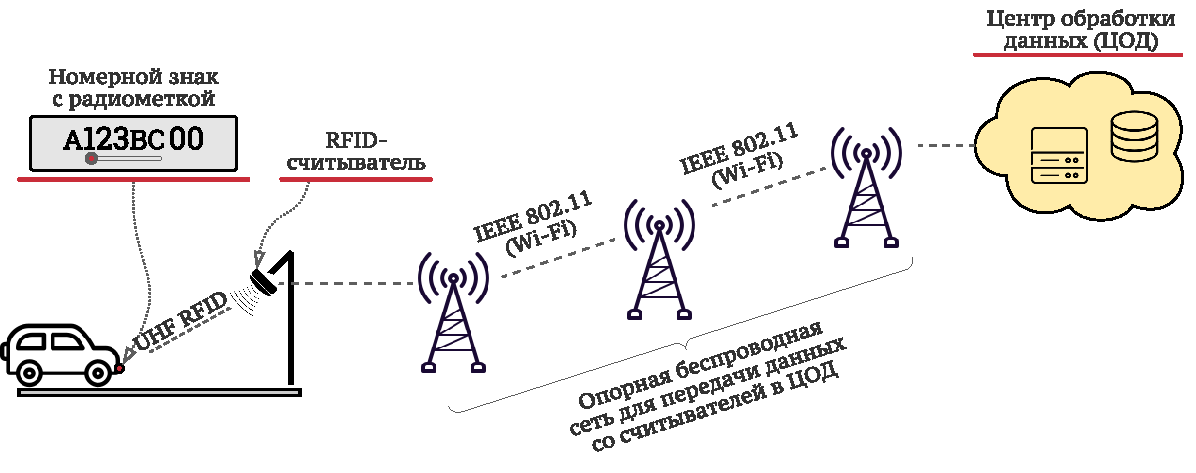
\includegraphics [scale=0.8] {chapter1/ch1_system_overview}
	\caption{Схема распределённой системы радиочастотной идентификации транспорта.}
	\label{fig:ch1_system_overview}
\end{figure}

Основными компонентами простейщей распределенной системы радиочастотной идентификации транспорта являются RFID-метки, RFID-считыватели, телекоммуникационная сеть и центр обработки данных. \textbf{RFID-метки} или \textbf{транспондеры} "--- это устройства, которыми оснащаются транспортные средства. Их назначение "--- передача записанного идентификатора считывателям. В зависимости от используемой технологии, могут быть активными или пассивными, то есть иметь или нет свой источник питания. Подробнее принцип работы меток стандарта EPC Class 1 Gen. 2 (ISO 18000-6C) описан в разделе~\ref{sec:ch1_rfid}. \textbf{RFID-считыватели} "--- активные устройства, осуществляющие чтение идентификаторов меток и их передачу в центр обработки данных. \textbf{Телекоммуникационная сеть} используется для передачи данных о метках от считывателей в центр обработки данных, а также для доступа администраторов к считывателям для их настройки, обслуживания и мониторинга. \textbf{Центр обработки данных} включает информационную систему, в которой собираются данные о прочитанных метках и состоянии работы считывателей.

В качестве примера можно привести системы для бесконтактного сбора оплаты проезда на автодорогах, например "--- на участках трасс М-4 <<Дон>>, М-1 <<Беларусь>> и Центральной кольцевой автодороге (ЦКАД). В некоторых странах (например, в Чили, ЮАР, Азербайджане) проводились эксперименты по более масштабному внедрению RFID, для регистрации всех или определенной группы автомобилей. Подобный эксперимент проводился и в России, в республике Татарстан, его результаты будут более подробно рассмотрены в настоящей работе.

Для получения данных о проезжающем транспортном средстве оно должно быть оснащено одной или несколькими RFID-метками, причем выбранная технология радиочастотной идентификации должна обеспечивать чтение метки на расстоянии 10--20 метров. Одной из наиболее подходящих технологий RFID, отвечающих этому требованию, является СВЧ-RFID стандарта EPC Class 1 Generation 2~\cite{StdGen2}, работающая в диапазоне 860--920 МГц. В частности, эта технология была использована в эксперименте, проведенном в городе Казань. В качестве альтернативы также можно использовать активные метки, или технологию DSRC, которая используется на уже упомянутых платных дорогах М-1, М-4 и ЦКАД.

%\subtodo{Добавить ссылки на DSRC и активные RFID}

Для передачи информации о считанных метках RFID-считыватели должны быть подключены к центрам обработки данных. Возможны три пути решения этой задачи: подключение к существующей проводной или беспроводной сети, коммутационное оборудование которой находится вблизи точек размещения считывателей; использование сотовой сети; построение отдельной сети для подключения считывателей. Использование существующих сетей оказывается не всегда возможным, особенно при развертывании системы за пределами крупных населённых пунктов. Кроме того, сети могут быть перегружены (например, если они уже используются для передачи данных с городских камер видеонаблюдения). Из-за ограниченности покрытия использование сотовой сети также не всегда возможно. В качестве примера, в настоящем исследовании будем рассматривать построение отдельной беспроводной сети. Как будет показано, для работы системы не нужно высокоскоростных каналов, и для подключения большого количества считывателей (порядка нескольких сотен) достаточно многошаговой сети, построенной на основе технологии IEEE 802.11g, оборудование которой очень недорогое и позволяет строить беспроводные соединения на расстояниях до нескольких десятков километров.

В центре обработки данных должна собираться как информация о зарегистрированных считывателями метках, так и о состоянии работы оборудования. Если в состав системы входят камеры, радары и прочее оборудование, в информационном центре можно объединять данные, полученные от различных источников. Например, объединяя результаты идентификации номерных знаков по фото с данными, полученными от считывателей, можно существенно повысить достоверность распознавания транспортного средства в условиях плохой видимости. Возможна интеграция и с системами приема оплаты или с базами розыска угнанных машин.

\begin{table}[ht!]
    \renewcommand{\arraystretch}{1.3}
    \caption{Технологии, используемые в распределённой системе радиочастотной идентификации транспорта, разработанной в рамках диссертационной работы.}
    \label{table:ch1_technologies}
	\begin{tabular}{ |p{0.17\linewidth}|p{0.26\linewidth}|p{0.47\linewidth}| }\hline
		Компонент & Технология & Комментарии\\\hline\hline
		Метки & EPC Class 1 Gen. 2 & Пассивные метки в номерных знаках или на стикерах под лобовым стеклом.\\\hline
		Считыватели & EPC Class 1 Gen. 2 & RFID-считыватели устанавливаются над дорогой, поддерживают до четырх антенн и подключаются к сети.\\\hline
		Сеть & IEEE 802.11 & Многошаговая беспроводная сеть с каналами, в которых используется схема доступа CSMA/CA.\\\hline
		ЦОД &  & Различное программное обеспечение для получения, сохранения и анализа данных о метках.\\\hline
	\end{tabular}
\end{table}

В ходе исследования, результаты которого приводятся в настоящей диссертационной работе, предполагалось, что для реализации распределённой системы радиочастотной идентификации транспорта используются технологии, описанные в табл.~\ref{table:ch1_technologies}.


% Следует оговориться, что в современных беспроводных сетях IEEE 802.11 используются гораздо более сложные и эффективные механизмы, нежели DCF, описываемый и исследуемый в настоящей работе; вместе с тем, механизм DCF гораздо проще для исследования, и, как будет показано в последующих главах, его вполне достаточно для эффективной реализации системы передачи данных со многих считывателей, что, вместе с низкой ценой соответствующего оборудования, делает его выбор вполне обоснованным для практической реализации.

% Технология радиочастотной идентификации далее рассматривается гораздо подробнее, чем протоколы передачи данных по беспроводным каналам. Это связано с тем, что вероятность идентификации движущихся меток, которая исследуется в следующих главах, существенно зависит от множества параметров протокола EPC Class 1 Generation 2. В то же время, при исследовании задержек в передаче данных по беспроводным каналам нас главным образом будет интересовать длительность обслуживания, в корректном моделировании которой заключается основная сложность работы, поэтому при описании протокола IEEEE 802.11 DCF мы сделаем акцент именно на временных аспектах работы и на механизме борьбы с коллизиями, игнорируя особенности кодирования и модуляции, а также прочие части протокола.




%%%%%%%%%%%%%%%%%%%%%%%%%%%%%%%%%%%%%%%%%%%%%%%%%%%%%%%%%%%%%%%%%%%%%%%%%%%%%%%%
\section{Постановка задач исследования}\label{sec:ch1_problems}
%%%%%%%%%%%%%%%%%%%%%%%%%%%%%%%%%%%%%%%%%%%%%%%%%%%%%%%%%%%%%%%%%%%%%%%%%%%%%%%%

При проектировании и построении распределённой системы радиочастотной идентификации транспорта возникает целый ряд задач, относящихся как непосредственно к идентификации транспорта, так и к организации связи между считывателями и центром обработки данных. Рассмотрим подробнее задачи, решению которых посвящена диссертационная работа.

%%% --------------------------------------------
\subsection{Исследование эффективности радиочастотной идентификации мобильных меток}
%%% --------------------------------------------

Критерием работоспособности системы является процент успешно распознанных транспортных средств. Задача осложняется тем, что метки могут двигаться с высокой скоростью (порядка 100--150~км/ч), а время, доступное для их чтения, крайне ограничено, так как считыватель может получить данные от метки лишь на небольшом расстоянии, порядка десяти метров. При различных настройках протокола EPC Class 1 Gen. 2 скорость обмена данными с меткой и вероятность успешной передачи сообщений могут меняться в очень широких пределах. Дополнительную сложность задаче придают многолучевое распространения сигналов между считывателем и меткой (как минимум, присутствие отраженного от дороги луча), наличие эффекта Доплера, а также использование метода обратного рассеяния для передачи ответов меток. Для решения задачи оценки работы системы радиочастотной идентификации удобно использовать методы имитационного моделирования, позволяющие учесть как параметры протокола, так и особенности распространения сигналов.

Отдельные аспекты работы считывателей можно исследовать с помощью методов теории случайных процессов. Хотя такой подход затрудняет учет всего объема факторов, влияющих на производительность системы, он позволяет более детально изучить отдельные закономерности, в частности "--- влияние периодических отключений питания и изменений подмножеств опрашиваемых меток на вероятность успешной идентификации. Для построения аналитической модели протокола нужно формально описать компоненты, определяющие состояние системы, а также формализовать операции, которые считыватель может осуществлять над метками. После этого можно исследовать свойства этих операций и найти способы получения оценки успешного чтения меток.

Таким образом, для исследования эффективности системы радиочастотной идентификации автомобилей нужно решить следующие задачи:

\begin{enumerate}
    \item Выявить факторы, влияющие на вероятность успешной идентификации мобильной RFID-метки.
    \item Построить формальную математическую модель системы радиочастотной идентификации, исследовать свойства операций, осуществляемых считывателем над множеством мобильных меток.
    \item Разработать аналитические и имитационные модели для получения оценки вероятности идентификации мобильных RFID-меток.
    \item Определить параметры протокола, при которых доля успешно идентифицированных автомобилей с RFID-метками оказывается не ниже 90\%.
\end{enumerate}

Решению этих задач посвящены главы 2 и 3 диссертации.



%%% --------------------------------------------
\subsection{Анализ производительности опорной сети}
%%% --------------------------------------------

Для работы некоторых приложений важно обеспечить быструю передачу информации о прочитанных метках в центр обработки данных. Например, это необходимо для реализации бесконтактной оплаты проезда или для поиска угнанных транспортных средств. Для анализа межконцевых задержек можно использовать как имитационное моделирование, так и аналитические модели, построенные на базе теории массового обслуживания.

Модели открытых тандемных сетей массового обслуживания хорошо известны и исследованы. Основная сложность их применения к задаче поиска межконецвых задержек пакетов, передаваемых в многошаговых сетях, заключается в выборе адекватных распределений интервалов между поступлениями пакетов в сеть и распределений длительности передачи пакетов по каналам связи.

В диссертационном исследовании предполагается, что опорная сеть строится на базе беспроводных линий связи с каналами CSMA/CA. Для моделирования каналов связи используются системы массового обслуживания MAP/PH/1/N, в которых интервалы между поступлениями пакетов в сеть моделируются марковскими случайными потоками (MAP), время обслуживания пакетов имеет распределение фазового типа (PH), а размер очереди ограничен. Получение численных характеристик открытых сетей MAP/PH/1/N $\rightarrow$ $\bullet$/PH/1/N $\rightarrow \dots \rightarrow \bullet$/PH/1/N осложняется экспоненциальным ростом пространства состояний при увеличении числа узлов в сети, и отдельной задачей является поиск эффективных способов получения численных оценок таких сетей.

Для оценки производительности опорной сети в диссертации решаются следующие задачи:

\begin{enumerate}
    \item Поиск PH-распределений, адекватно моделирующих время обслуживания в беспроводных сетях с каналами CSMA/CA.
    \item Оценка возможности использования метода аппроксимации выходящих потоков для получения численных оценок межконцевых задержек в открытых тандемных сетях массового обслуживания с узлами типа MAP/PH/1/N.
    \item Получение численных оценок межконецвых задержек для многошаговой беспроводной сети с помощью аналитического и имитационного моделирования.
\end{enumerate}

Решению этих задач посвящена глава 4 диссертации.


%%% --------------------------------------------
\subsection{Экспериментальная реализация системы}
%%% --------------------------------------------

Для того, чтобы исследовать работоспособность системы радиочастотной идентификации автомобилей, были разработаны экспериментальные RFID-считыватели, распределенная система управления считывателями и программное обеспечение для центров обработки данных. Разработанный программно-аппаратный комплекс проходил испытания в трех экспериментах. Первый эксперимент прошел в 2014--2015 годах в городе Казань. Тогда метками были оснащены около 750 автобусов, в двух точках города установлены RFID-считыватели, информация с которых передавалась в центр обработки данных в ГИБДД. За несколько зимних месяцев была собрана статистика, вероятность идентификации составила 92--95~\%. Следующий эксперимент проходил в 2020 году также в Казани, его целью была проверка системы при идентификации автомобилей, движущихся со скоростями до 170~км/ч и совершающих различные маневры. Третий эксперимент начался летом 2021 года на ЦКАД, его целью была проверка применимости системы для сбора данных для оплаты проезда. Все эксперименты завершились успешно.

При разработке программного обеспечения RFID-считывателей требовалось обеспечить его высокую надежность, быстродействие, а также гибкость. В частности, было принято решение разделить потоки данных и управления (сигнализации) так, чтобы, с одной стороны, сделать невозможным изменение параметров работы считывателя каким-либо образом, кроме как через административный интерфейс, а с другой стороны "--- упростить подключение внешних клиентов для получения потоков считанных меток. Программное обеспечение было спроектировано таким образом, чтобы можно было в быстро заменить радиомодули RFID-считывателей без изменения кода остальных компонентов, а также обеспечить возможность выноса части компонентов за пределы считывателя.

В состав разработанного программного обеспечения входит управляющий модуль (супервайзер), адаптеры радиомодулей, интерфейсы управления (веб-интерфейс, интерфейс командной строки), а также модули для приема и обработки потоков данных о прочитанных метках. Все программное обеспечение, за исключением веб-интерфейса, было реализовано на языках C и C++.

Для экспериментального исследования производительности системы радиочастотной идентификации были решены следующие задачи:

\begin{enumerate}
	\item Разработка архитектуры распределённой системы управления RFID-считывателями и протоколов связи между компонентами системы.
	\item Программная реализация распределённой системы управления и разработка программного обеспечения для приема, обработки и записи данных о прочитанных метках.
	\item Проведение экспериментальных исследований и получение оценки вероятности успешной идентификации автомобилей при различных скоростях движения, маневрах, погодных условиях.
\end{enumerate}

Решению этих задач посвящена глава 5 диссертации.



%%%%%%%%%%%%%%%%%%%%%%%%%%%%%%%%%%%%%%%%%%%%%%%%%%%%%%%%%%%%%%%%%%%%%%%%%%%%%%%%
\section{Радиочастотная идентификация транспортных средств}\label{sec:ch1_rfid}
%%%%%%%%%%%%%%%%%%%%%%%%%%%%%%%%%%%%%%%%%%%%%%%%%%%%%%%%%%%%%%%%%%%%%%%%%%%%%%%%

Технология радиочастотной идентификации (RFID) является альтернативой для традиционной идентификации номеров транспортных средств по фото. Для использования этой технологии автомобили оснащаются радиометками, а в точках контроля размещаются считыватели. Когда метка проезжает мимо считывателя, она передает свой идентификатор, по которому определяется номер автомобиля. К преимуществам этой технологии относится относительно низкая стоимость оборудования, низкие требования к пропускной способности каналов связи, отсутствие необходимости в частом обслуживании и слабая зависимость от погодных условий.

Существует несколько различных технологий радиочастотной идентификации. В \textbf{активных} системах используются метки, обладающие собственным источником питания. Часто такие системы работают в диапазоне 2.4 ГГц и могут быть основаны, например, на технологиях IEEE 802.11 (WiFi) или ZigBee. Можно выделить технологию DSRC (Dedicated Short-Range Communication), которая часто используется в системах оплаты проезда по автомагистралям, в том числе и в России. Дальность действия считывателя в системах с активными метками может достигать десятков или даже сотен метров, но метки достаточно громоздки и дорогостоящи.

К другому классу относятся \textbf{пассивные} системы, в которых метки не обладают собственными источниками энергии. Для работы и передачи данных метки в таких системах используют энергию, получаемую из электромагнитного поля, создаваемого считывателем. RFID-системы LF-диапазона (125 "--- 134 кГц, ISO/IEC 18000-2) характеризуются малым расстоянием идентификации (порядка нескольких сантиметров) и используются, например, для чипирования животных. Системы HF-диапазона (13,56 МГц, стандарты ISO/IEC 18000-3, ISO/IEC 15693, ISO/IEC 14443 A,B) очень широко распространены в области электронной оплаты (например, оплата проезда на общественном транспорте) и контроля доступа, характеризуются низкой стоимостью и дальностью порядка нескольких миллиметров или сантиметров. Системы UHF-диапазона (860 "--- 960 МГц, ISO/IEC 18000-6C, EPC Gen-2) работают на расстояниях до 15--20 метров и используются в логистике, торговле, контроле доступа и на производствах. Кроме того, метки UHF-диапазона иногда оснащаются собственным источником питания, который может использоваться для работы встроенного сенсора. В этом случае метка может передавать результаты измерений, полученные от сенсора, а питание также может использоваться для усиления отражаемых сигналов. Такие метки называются полупассивными или полуактивными.


%%% --------------------------------------------
\subsection{Стандарт EPC Class 1 Generation 2}\label{sec:ch1_rfid_std}
%%% --------------------------------------------

Стандарт EPC Class 1 Generation 2~\cite{StdGen2} (ISO/IEC 18000-6C, ГОСТ Р 58701-2019 \cite{GostRfid}) описывает физический (PHY) и канальный (MAC) уровни системы радиочастотной идентификации пассивных и полупассивных меток. На физическом уровне стандарт описывает способы модуляции и кодирования сигналов, а на канальном уровне "--- протокол обмена данными между считывателем и метками. Протокол основан на Slotted ALOHA \cite{Abramson1970, Roberts1975}, позволяет бороться с коллизиями при нахождении нескольких меток в зоне считывателя, а также содержит средства для чтения и записи данных на метки.

Поскольку пассивные метки не имеют собственного источника питания, счиытватель постоянно создает электромагнитное поле, которое используется метками для получения энергии. Периодически считыватель отключает питание, обеспечивая меткам возможность сбросить некоторые регистры и флаги. В то время, когда считыватель не осуществляет передачу своих команд, он генерирует синусоидальный сигнал (Constant Wave, CW), который метки используют в качестве несущей "--- для передачи ответов метки модулируют отражаемый ими сигнал CW, полученный от считывателя, изменением своего коэффициента отражения (т.е. передача данных от меток ведётся методом обратного рассеяния).

Метки не могут сами инициировать обмен данными со считывателем, они всегда передают свои сообщения в ответ на получаемые от считывателя команды. Стандарт допускает следующие основные действия с меткой: инвентаризацию, чтение, запись и блокирование памяти, а также уничтожение метки. Инвентаризация "--- это опрос меток, в ходе которого они передают считывателю свои идентификаторы EPCID и выполняют другие операции, которые может запросить считыватель.  Блокирование памяти означает, что считыватель впоследствии не сможет записать эту область памяти. Наконец, операция уничтожения метки приводит к тому, что в будущем метка никогда не будет участвовать в инвентаризации. Протокол определяет и другие операции, включая средства для защиты доступа к данным. Производители могут реализовать дополнительные операции на своих метках. В рамках диссертационной работы интерес будут представлять только инвентаризация и чтение памяти.


%%% ~~~~~~~~~~~
\subsubsection{Логическая структура памяти метки}\label{sec:ch1_rfid_std_memory}
%%% ~~~~~~~~~~~

Каждая метка включает в себя четыре банка памяти (см. рис. \ref{fig:ch1_banks}): EPC, TID, зарезервированную память (Reserved) и пользовательскую память (User).

\begin{figure}[ht]
  \centering
  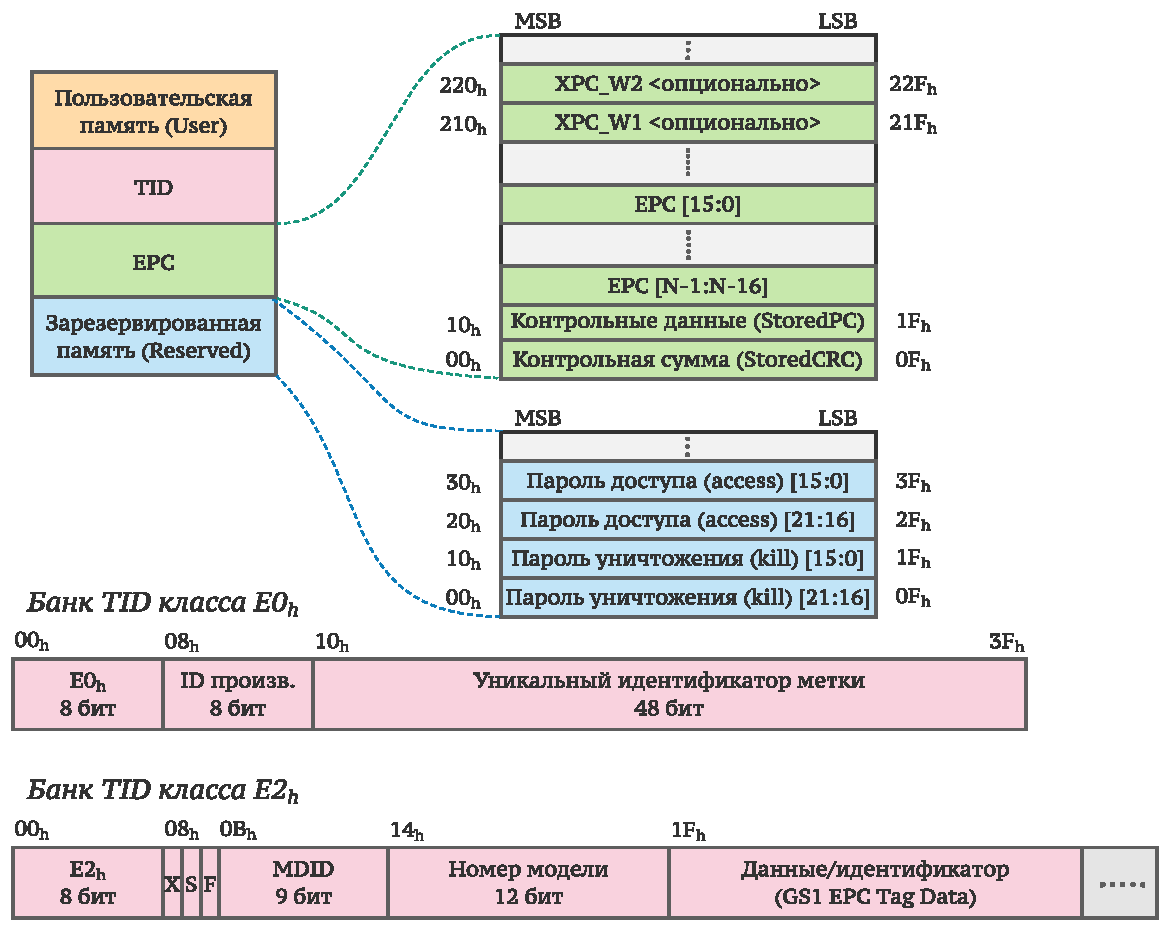
\includegraphics [scale=0.8] {chapter1/ch1_banks}
  \caption{Логическая структура памяти метки}
  \label{fig:ch1_banks}
\end{figure}

Банк EPC содержит код EPC (Electronic Product Code), контрольную сумму (StoredCRC) и служебную информацию (PC, Protocol Control), в которой хранятся данные о длине поля EPC, доступности пользовательской памяти и прочую информацию. Объем памяти в поле EPC может меняться от метки к метке, распространненым значением является 96 бит. Чтобы не путать название банка памяти и значение EPC, значение в дальнейшем будем называть EPCID.

Банк Reserved хранит пароли для блокирования и уничтожения меток, если метка поддерживает соответствующие операции.

Банк TID хранит данные о производителе и модели метки, а также ее уникальный идентификатор. Главная особенность банка TID "--- фабричная защита от изменений значения, записанного при производстве метки, поэтому его удобно использовать в задаче надежной идентификации объектов. Первые 8 бит TID содержат идентификатор класса, который может быть равен либо $\text{E0}_\text{h}$, либо $\text{E2}_\text{h}$. Если идентификатор класса равен $\text{E0}_\text{h}$, то длина банка равна 64 битам, второй октет содержит идентификатор производителя, а последние 48 бит содержат серийный номер метки. Такие метки производства NXP использовались в эксперименте в Казани в 2014 году. Структура банка TID для класса $\text{E2}_\text{h}$ более сложная, а его размер "--- больше. Следюущие после первого октета три бита "--- служебные флаги, после них "--- 9-битный идентификатор производителя MDID (Mask Designer Identifier), далее 12-битный номер модели и уже после него уникальный номер метки. Например, метки производства АО <<Микрон>>, которые использовались в экспериментах 2020-го и 2021-го года, имеют класс $\text{E2}_\text{h}$ и содержат 96-битные значения.

Банк пользовательской памяти может иметь достаточно большой объем (порядка 512 бит) и используется для хранения дополнительных данных, например "--- подробной информации о маркированном предмете.


%%% ~~~~~~~~~~~
\subsubsection{Физический уровень}\label{sec:ch1_rfid_std_phy}
%%% ~~~~~~~~~~~

При передаче данных от считывателя к меткам используется амплитудную модуляцию DSB-ASK, SSB-ASK или PR-ASK. Для кодирования используется схема PIE (Pulse Interval Encoding), в которой нули и единицы кодируются символами data-0 и data-1 различной длины (см. рис.~\ref{fig:ch1_pie}).

\begin{figure}[ht]
  \centering
  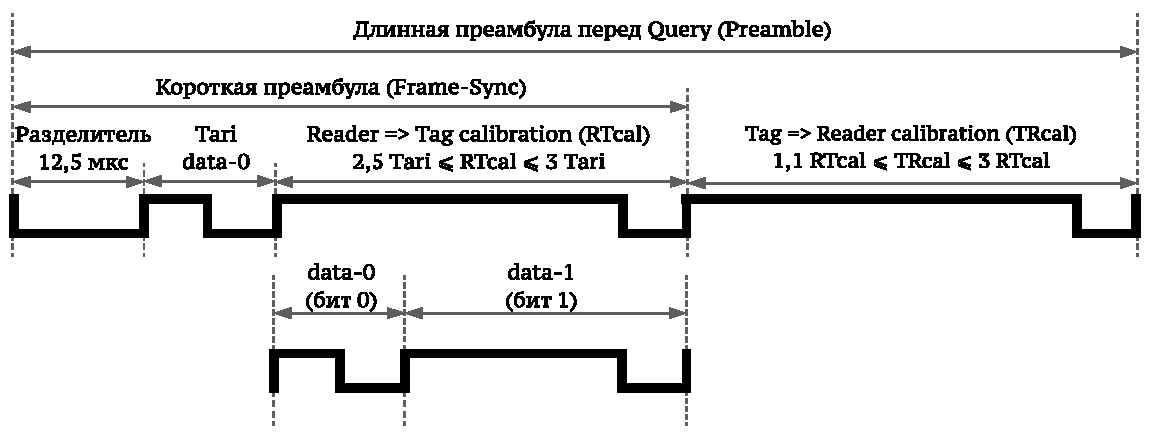
\includegraphics [scale=0.8] {chapter1/ch1_pie}
  \caption{Символы в схеме PIE и преамбулы команд RFID-считывателя}
  \label{fig:ch1_pie}
\end{figure}

Передачу каждой команды считыватель начинает с синхронизирующей последовательности (преамбулы). Стандарт определяет два вида преамбул (см. рис.~\ref{fig:ch1_pie}): длинную, называемую в стандарте преамбулой, и короткую, называемую синхронизацией кадра, (Frame-Sync). Оба вида преамбул начинаются с постоянного разделителя длительностью 12,5~мкс, за ним идут символы ноль (data-0) и RTcal (Reader-to-Tag calibration). Длительность символа data-0 называется Tari. Длительность символа RTcal равна суммарной длительности нуля и единицы, этот символ используется меткой для различения символов data-0 и data-1: если символ короче половины RTcal, то это ноль, иначе "--- единица. Короткая преамбула завершается передачей RTcal, а длинная содержит также символ TRcal (Tag-to-Reader calibration), длительность которого используется меткой для расчета скорости, с которой она должна передавать свой ответ.

Длинная преамбула отличается от короткой наличием символа TRcal и передается перед первой командой Query, с которой считыватель начинает опрос меток. Так как метка, не получившая Query, все равно не сможет участвовать в опросе, передавать TRcal в последующих кадрах не имеет смысла и используется короткая преамбула, содержащая только ту информацию, которая нужна метке для успешного декодирования команды.

Отметим, что из-за использования PIE длительность кадров, передаваемых считывателем, зависит от числа нулей и единиц в команде. Поэтому для точного моделирования протокола необходимо учитывать результат кодирования команд.

Метка передает свой ответ, модулируя несущую, полученную от считывателя. Метка может использовать амплитудную (ASK) или фазовую (PSK) модуляцию. В качестве схемы кодирования используется либо код FM0, либо коды Миллера с 2, 4 или 8 символами на бит. Все схемы кодирования, поддерживаемые метками, имеют память, то есть вид символа, кодирующего следующий бит, определяется предыдущим битом. Перед передачей ответа метка передаёт преамбулу, которая может быть обычной или расширенной. Короткая преамбула равна по длительности 6 битам для кода FM0 и 10 битам для кодов Миллера, а расширенная - 18 и 22 битам соответственно. Кроме того, после каждого ответа метки следует символ, не кодирующий ни ноль, ни единицу.

Для вычисления скорости передачи символов метка вычисляет величину BLF (Backscatter Link Frequency) по следующей формуле:

$$
\text{BLF} = \frac{\text{DR}}{\text{TRcal}},
$$
где DR (Divide Ratio) - величина, передаваемая в команде Query, и принимающая одно из двух значений: 8 или 64/3. Для вычисления битовой скорости необходимо разделить BLF на число символов на бит в используемом меткой методе кодирования (M=1,2,4,8). В отличие от считывателей, использующих PIE, все биты в ответах меток имеют одинаковую длительность, поэтому их содержание не оказывает влияния на длительность передачи ответов.



%%% ~~~~~~~~~~~
\subsubsection{Логический уровень}\label{sec:ch1_rfid_std_logic}
%%% ~~~~~~~~~~~

Протокол доступа к каналу, описываемый в стандарте \cite{StdGen2}, основан на протоколе Framed Slotted ALOHA \cite{Roberts1975, Abramson1970}. Все время работы разбито на \textbf{раунды} (см. рис. \ref{fig:ch1_inventory}), которые начинаются передачей считывателем команды Query. Эта команда, среди прочего, несет в себе параметр Q, который используется метками для расчета количества слотов в раунде как $2^\text{Q}$. Получив Query, метка выбирает случайный номер слота \textit{SN} для передачи своего ответа от 0 до $2^\text{Q}-1$. При последующем получении команд QueryRep метка уменьшает значение счетчика \textit{SN}. Когда счетчик доходит до 0, метка генерирует и передает случайное 16-битное число (RN16). Считыватель, получив это случайное число, пересылает его в команде Ack. Метка сравнивает полученное значение с отправленным. Если значения совпадают, то в ответ на Ack метка пересылает свой EPCID с контрольной суммой (PacketCRC) и контрольными данными (PC). Если же значения не совпадают, метка считает, что Ack предназначен не ей, и ничего не отвечает.

\begin{figure}[ht]
  \centering
   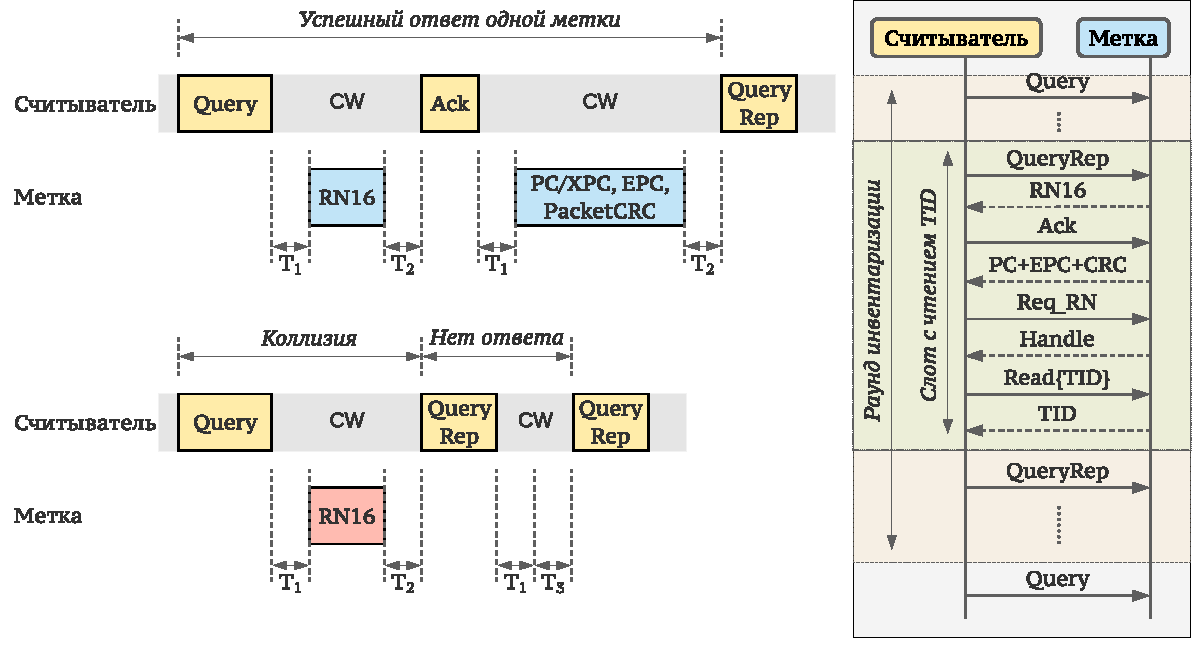
\includegraphics [scale=0.8] {chapter1/ch1_inventory}
  \caption{Схема опроса меток и раунд инвентаризации}
  \label{fig:ch1_inventory}
\end{figure}

Стандарт определяет границы интервалов, которые должны пройти между последовательными командами и ответами:

\begin{itemize}
	\item $T_1$: минимальное время между концом последнего символа команды и первым символом преамбулы ответа;
	\item $T_2$: минимальное время между окончанием последнего (псевдо-) бита ответа метки и первым символом преамбулы команды считывателя;
	\item $T_3$: минимальный интервал между окончанием $T_1$ и следующей командой считывателя.
\end{itemize}

Все, что происходит от передачи QueryRep до получения ответа от метки с EPCID, называется \textit{стадией инвентаризации}. Именно в ней разрешаются коллизии "--- если несколько меток выбрали один слот и одновременно передали слова RN16, то считыватель, скорее всего, не сможет получить ни одно из них и либо вовсе не отправит Ack, либо отправит Ack с неправильным значением. Если же метка получила Ack с правильным значением, то коллизии не было, поэтому она может передать более длинное (по сравнению с RN16) значение EPCID. Если считыватель смог обнаружить ошибку в ответе метки, он может передать команду NACK, получив которую метка сможет определить, что ее идентификатор не был успешно передан. Также считыватель может повторно отправить Ack, чтобы метка повторила передачу EPCID.

Если после получения EPCID считывателю нужно выполнить над меткой другие действия, он начинает \textit{стадию доступа}. В ней он запрашивает новое случайное число от метки с помощью команды Req\_RN и, после получения ответа, передает команду чтения, записи, блокирования или уничтожения метки. Если метка использует пароль для доступа, то перед передачей команды считыватель должен отправить пароль.

Помимо стадий инвентаризации и доступа, стандарт определяет \textit{стадию выбора}. До отправки команды Query считыватель может передать команду Select, в которой задать параметры тех меток, ответы от которых он хочет получить в текущем раунде. Эту команду удобно использовать при опросе большого числа меток, например на складе. Еще одна интересная особенность стандарта "--- возможность динамически изменять число слотов. Если считыватель обнаруживает, что коллизии происходят слишком часто или, наоборот, слишком много пустых слотов, он может передать команду QueryAdjust с новым значением Q и запросить метки, которые еще не ответили в этом раунде, выбрать новые слоты. Подробнее про протокол взаимодействия между считывателями и метками можно прочитать в стандарте~\cite{StdGen2}.

В диссертационной работе будет использоваться фиксированное значение Q и только одна операция доступа "--- чтение банка TID. Для ее выполнения считыватель использует команду Read, в которой отмечает нужный банк (TID), адрес начала памяти ($\text{00}_\text{h}$) и число 16-битных слов, которые нужно прочитать. Если команда выполнена успешно, метка передает в ответ хранящееся значение. Пример чтения банка TID показан на рис.~\ref{fig:ch1_inventory}.



%%% ~~~~~~~~~~~
\subsubsection{Сессии}\label{sec:ch1_rfid_std_sessions}
%%% ~~~~~~~~~~~

Сессии позволяют разграничить множество окружающих считыватель меток. Каждая метка должна поддерживать четыре сессии S0, S1, S2 и S3. Для каждой сессии метка имеет отдельный флаг, значения которого в стандарте обозначаются как $A$ и $B$.

В команде Query считыватель указывает, с какой сессией работает в этом раунде, и какое значение флага сессии должно быть у меток, которые могут участвовать в опросе. После передачи EPCID метка, получив команду Query, QueryRep или QueryAdjust, должна инвертировать хранящееся у нее значение флага ($A \rightarrow B$, $B \rightarrow A$). Если в следующем раунде опрос будет проходить по той же сессии и тому же значению флага, эта метка участвовать в раунде не будет, так как у нее хранится инвертированное значение флага. Если считыватель не смог получить EPCID, он может передать команду NAK "--- в этом случае метка не изменит флаг и сможет участвовать в следующем раунде.

Сессии различаются по требованиям ко времени сохранения значения флага при потере питания, а также к начальным значениям флагов. Флаг сессии S0 всегда инициализируется в значение $A$. Он сбрасывается всякий раз, когда метка теряет питание. Флаг сессии S1 сбрасывается в значение $A$ при включении метки, если со времени его изменения прошло не менее интервала, значение которого может варьироваться от 0,5 с до 5~с. Значение также сбрасывается в том случае, если метка не выключалась и с момента последнего изменения прошло слишком много времени. Флаги сессий S2 и S3 должны сбрасываться в $A$, если с момента выключения метки прошло не менее 2~с. Таким образом, использование сессий S2 и S3 может предотвратить изменение флага в случае краткосрочной потери меткой энергии.

Как будет подробно исследовано в главе 3, выбор сессии и сценария опроса (всегда ли опрашивать метки по значению флага $A$ или чередовать опросы по $A$ и по $B$) оказывает существенное влияние на вероятность успешной идентификации метки.



%%% --------------------------------------------
\subsection{Обзор исследований производительности UHF RFID}\label{sec:ch1_rfid_observe}
%%% --------------------------------------------

Технология радиочастотной идентификации \cite{Finkenzeller2010, Dobkin2008} используется во множестве приложений, от учета товаров на складах, до поиска автомобилей на парковке с помощью дронов \cite{Wu2019}, позиционирования мобильных объектов \cite{Cho2013, Park2013, Errington2010}, расчета скорости движущихся автомобилей \cite{Zhai2018, Choy2020, Jing2013}, и даже выявления признаков усталости водителя \cite{Yang2020} (в последнем случае метки предлагается размещать с двух сторон на шапке), или оперативного поиска потервшихся в городе людей (например, с болезнью Альцгеймера или иными расстройствами) с помощью RFID-считывателей на припаркованных автомобилях \cite{Griggs2018}.

Задача идентификации транспорта является одним из основных применений RFID \cite{StdRainEviWhitepaper}. Первые системы сбора платы за проезд, использующие RFID, появились в США в 1991 году \cite{Landt2005}. Использование RFID для идентификации автомобильного и железнодорожного транспорта исследовалось в работах \cite{Gonzalez2013, Blythe1999, Khan2011, Yoon2008, Al-Naima2011, Tseng2007, Kostrominov2020, Unterhuber2019, Unterhuber2020, Unterhuber2019, Pawowicz2020, Choy2020, Jo2009, Zhang2010, MenesesGonzalez2011, Lonkar2018, Balbin2017, Bhavke2017, Zhang2011, Zhang2010a, Pandit2009, Sundar2015}. В частности, в работе \cite{Unterhuber2020} Unterhuber и соавторы рассматривают систему идентификации быстрого транспорта (автомобилей и поездов) и утверждают, что наиболее критичный параметр, определяющий вероятность идентификации "--- число раундов, в которых успевает принять участие метка. Авторы предлагают простую модель для оценки максимального числа раундов, используют реалистичные модели антенных систем и получают результаты, доказывающие, что UHF RFID можно применять для идентификации очень быстро движущихся автомобилей и поездов. Unterhuber и соавторы также отмечают, что из-за многолучевого распространения и эффекта Доплера может существовать несколько отрезков, на которых возможна идентификация (аналогичные данные получены в моделях, представленных в диссертации). Вместе с тем, в работе \cite{Unterhuber2020} не рассматриваются коллизии или идентификация меток по TID. Стоит также выделить предыдущую работу Unterhuber и соавторов \cite{Unterhuber2019} и работу Marais и соавторов \cite{Marais2013}, в которых представлен анализ оптимального угла наклона антенн при идентификации транспорта.

Использование RFID в рамках интеллектуальных транспортных систем и <<умных городов>> "--- одно из перспективных направлений исследований \cite{Pawowicz2020, Pandit2009, Sundar2015}. Например, Pawłowicz и соавторы в работе \cite{Pawowicz2020} рассматривают задачу идентификации транспортного потока в контексте концепции <<умного города>>, предлагают очень простую аналитическую модель и сравнивают данные, полученные с ее помощью, с результатами макетного моделирования.

Процесс чтения движущихся меток, в общем случае, не является надежным "--- метка может быть потеряна из-за высокой скорости движения, слабого сигнала или коллизий. Для того, чтобы предсказать, будет ли идентифицирована метка, и извлечь дополнительную информацию из данных, полученных от считывателя, можно использовать методы машинного обучения. В работе \cite{Jo2009} Jo и соавторы используют метод опорных векторов (SVM) для предсказания того, будет ли идентифицирован движущийся объект, в зависимости от скорости, угла наклона антенны и положения метки. А в работе \cite{Choy2020} Choy и соавторы используют искусственные нейронные сети для вычисления скорости движения автомобилей по мощности принятого RFID-считывателем сигнала. В работе также отмечено, что основная задача "--- борьба с нарушениями скоростного режима, а метки желательно размещать в номерах автомобилей.

Применение пассивных и активных RFID-тенхологий на дорогах не ограничивается простой идентификацией транспорта. Так, в работах \cite{GarciaOya2018, Jing2016, Hidalgo2013, Jing2013, Cheng2012, Perez2010} предлагается использовать RFID для чтения данных с дорожных знаков или с дорожного полотна. В этом случае метки располагаются на статичных объектах, а считыватели "--- в автомобилях. А в работе \cite{Porter2008} Porter и Kim описывают результаты эксперимента, проведенного в штате Орегон (США), в ходе которого RFID-метки использовались для сбора и передачи данных о пройденным автомобилем пути для дальнейшего расчета налога на топливо при заправке "--- авторы совместно с управлением транспорта штата Орегон исследовали возможность гибкого расчета топливного сбора на основе пройденного автомобилем расстояния. Отметим, что в этой работе использовался RFID в диапазоне 2,4~ГГц с доступом к каналу CSMA/CA. В работах \cite{Zheng2020, HongziZhu2009, Pandit2009} предлагается использовать информацию, полученную при чтении меток, для анализа трафика и траекторий передвижения, позиционирования и поиска угнанных автомобилей. Отметим, что в работе \cite{HongziZhu2009} предполагается использование активных RFID в диапазоне 2,4~ГГц.

Некоторые исследователи предлагают устанавливать пассивные RFID-метки в дорожное покрытие и использовать их для измерения скорости движения или передачи данных автомобилям, оборудованным RFID-считывателем. Cheng и соавторы \cite{Cheng2012} предлагают использовать такие дорожные метки для позиционирования автомобилей. Jing и соавторы \cite{Jing2016} также предлагают размещать метки на полосах движения и использовать их не только для передачи статических данных автомобилям (местоположение, направление движения, ограничение скорости и пр.), но и для записи автомобилями данных о текущей обстановке; эти данные затем могут быть получены другими проезжающими автомобилями, как от меток, так и в результате передачи данных по беспроводной сети между машинами. В работе \cite{Jing2013} Jing и соавторы приводят простой расчет минимального расстояния между метками, при котором водители с агрессивной манерой вождения не смогут ускориться и замедлиться так, чтобы их мгновенная скорость существенно превышала ограничение, но средняя скорость оставалась допустимой.

Отметим, что протокол, лежащий в основе канального уровня стандарта EPC Gen-2 \cite{StdGen2} "--- Framed Slotted ALOHA \cite{Abramson1970}. Исходный протокол ALOHA был представлен в работе \cite{Roberts1975}. В этой же работе, на основе предположения о пуассоновском потоке передаваемых пакетов, была получена оценка пиковой пропускной способности сети как $1/(2e) \approx 0,186$. Позднее, в работе \cite{Abramson1970} был описан способ повышения пропускной способности в два раза за счет разбиения времени на слоты (Slotted ALOHA).

Ряд работ посвящен имитационному моделированию систем UHF RFID \cite{Floerkemeier2009, Arnitz2009, Zhang2010, Jing2016}. Так, в работе \cite{Floerkemeier2009} была предложена модель JiST, реализованная на языке Java; в работе описывается дизайн системы моделирования и ее применение. К сожалению, симулятор JiST давно не обновлялся и, судя по всему, в настоящее время практически не используется. В работе \cite{Arnitz2009} сделан фокус на особенности распространения сигналов, моделировании каналов передачи данных и прочих низкоуровневых особенностях RFID-системы, однако практически не учитываются аспекты верхнего (логического) уровня. Авторы работы \cite{Zhang2010} предлагают использовать комбинацию симулятора OMNeT++ для моделирования логики и MATLAB для моделирования физического уровня, в качестве примера рассматривают модель UHF RFID. В работе \cite{Jing2016} также упоминается имитационная модель RFID, разработанная в системе моделирования OMNeT++.

Для того, чтобы адекватно моделировать процесс обмена сообщениями, учитывая потери из-за ненадежности каналов связи между считывателем и меткой, требуется детально учитывать особенности антенных систем, чувствительность меток и считывателя и свойства распространения сигналов. Эти вопросы изучлись во многих работах, в том числе в \cite{Dimitriou2014, Azpilicueta2016,  Griffin2009,  Nikitin2012, Nikitin2009, Nikitin2008, Nikitin2007, Nikitin2006, Nikitin2006a, Rao2005, Zanetti2010}. Работы \cite{Dimitriou2014, Azpilicueta2016} предлагают модели распространения сигналов, основанные на технике трассировки лучей. Авторы работы \cite{Dimitriou2014} рассматривают особенности распространения сигналов внутри помещений со множеством отражений, однако акцентируются на стационарных объектах и игнорируют эффект Доплера. В работе \cite{Azpilicueta2016} авторы моделируют систему с движущимися транспортными средствами, однако не учитывают параметры логического уровня и фокусируются на оценке энергетических параметров в сравнении с данными, полученными из эксперимента. В работах \cite{Nikitin2008, Griffin2009} предложена точная модель для расчёта бюджета соединений. В работе \cite{Nikitin2008} Никитин и Рао рассматривают возможные конфигурации антенн считывателей, приводят типичные значения SNR для различных компонентов антенных систем считывателя, демонстрируют существенные различия в расчете затухания сигнала для однолучевой и многолучевой моделей, приводят формулы для расчета бюджета соединений, а также приводят результаты измерений для различных меток. Кроме того, авторы отмечают, что основной вклад в шум при приеме ответов считывателем вносит не термический шум, а утечка излучаемого сигнала. В диссертационной работе этот факт будет использоваться при расчете SNR.

Влияние коллизий и расчет BER рассматривается в работе Lazaro и соавторов \cite{Lazaro2009}. Авторы предлагают для расчета BER использовать не обычную модель канала с аддитивным Гауссовым шумом (AWGN), а модель, полученную из AWGN усреднением по соотношению SNR, которое предполагается случайным, имеющим распределение Рэлея.

Значительное число работ посвящено анализу производительности систем радиочастотной идентификации. Авторы пользуются эмпирическими методами \cite{Buettner2008}, используют аппарат марковских случайных процессов как с идеальным каналом \cite{Vogt2002, Wang2009, Vahedi2012, Vales-Alonso2009, Vales-Alonso2011, Tong2007, Vales-Alonso2017}, так и с каналом с ошибками \cite{DiMarco2014}, а также используют иные аналитические подходы для анализа производительности \cite{Ahmed2016, Yan2014, Jeon2009, Kim2007}. В ряде работ также сравнивается производительность протокола Frame Slotted ALOHA с альтернативными протоколами и расширениями \cite{Vahedi2014, LaPorta2011}. В работе \cite{Buettner2008} M. Buettner пришел к выводу, среди прочего, что в ряде случаев при опросе выгоднее не пересылать повторно команды ACK при потере ответа от метки, а лучше выключиться и попробовать в следующем раунде или использовать иную стратегию опроса. Аналогичный подход будет использоваться в диссертационном исследовании. Отметим также работу \cite{Vales-Alonso2017}, в которой с помощью дискретной цепи Маркова исследуется эффект потери метками питания. Авторы описывают систему в виде двумерной цепи, моделируя изменение числа меток, которые продолжают участвовать в опросе, и число меток, уже передавших свои данные. В результате проведенного анализа, авторы находят оценки вероятности идентификации к концу раунда опроса и пропускную способность системы. В отличие от представленных в диссертационной работе моделей, потери пакетов возникают только вследствие коллизий, не учитываются сессии, и моделирование производится по слотами в одном раунде, а не по раундам. Также стоит выделить работу \cite{Pawowicz2020}, в которой предлагается очень простая модель для оценки вероятности потери метки, то есть ее проезда области чтения без идентификации. Авторы делят область чтения на сегменты фиксированной длины и, полагая, что передавшие свой идентификактор метки не участвуют в последующих раундах, предлагают простой метод расчета. Как и в главе 3 диссертационного исследования, авторы \cite{Pawowicz2020} рассматривают изменения системы между раундами, в том числе "--- поступления и выходы метки из области чтения. В то же время, степень детализации модели в диссертационном исследовании существенно выше.

Модель системы радиочастотной идентификации транспорта, описанная в главе 2, в значительной степени опирается на результаты, описанные в работах Никитина и Рао \cite{Nikitin2008}, Lazaro \cite{Lazaro2009}, Griffin \cite{Griffin2009} и других. Новизна предложенной в диссертации модели заключается в совместном моделировании как особенностей радиопередачи (включая эффект Доплера и многолучевое распространение), так и антиколлизионного протокола в единой имитационной модели и получении из нее оценок вероятности идентификации автомобилей по паре меток. Кроме того, в большинстве работ не рассматривается идентификация по TID, которая исследуется в диссертационной работе.

Аналитическая модель, описанная в главе 3, также имеет ряд отличий от существующих исследований. Во-первых, переходы марковской цепи происходят на границах раундов, а не слотов, и учитывают сбросы питания и смены флагов опроса меток. Во-вторых, модель учитывает потери произвольных пакетов из-за ненулевой битовой ошибки. В-третьих, модель состоит из двух марковский процессов, первый из которых нужен для расчета числа меток, участвующих в раундах, а второй "--- для оценки вероятности идентификации. В-четвертых, матрицы переходных вероятностей строятся в виде произведения матриц отдельных операций (проведение опроса, инвертирование флага опроса, сброс питания, добавление или удаление метки из области чтения). Из-за этого марковские процессы оказываются неоднородными и тяжелее в анализе, но предложенный метод становится очень гибким. В дальнейшем метод можно расширить на более сложные операции.




%%%%%%%%%%%%%%%%%%%%%%%%%%%%%%%%%%%%%%%%%%%%%%%%%%%%%%%%%%%%%%%%%%%%%%%%%%%%%%%%
\section{Передача данных по беспроводным сетям}\label{sec:ch1_wifi}
%%%%%%%%%%%%%%%%%%%%%%%%%%%%%%%%%%%%%%%%%%%%%%%%%%%%%%%%%%%%%%%%%%%%%%%%%%%%%%%%

Исторически, одним из первых методов доступа к каналу стал CSMA/CA, который был взят за основу уже в первых версиях стандарта IEEE 802.11. Базовый механизм доступа, описанный в этом стандарте и основанный на CSMA/CA, называется DCF (Distributed Coordination Function). Хотя современные версии стандарта используют гораздо более совершенные методы конкурентного доступа, позволяющие учитывать QoS, производить групповые передачи, подтверждать группы пакетов вместо отдельных, объединять каналы и пр., так или иначе в их основе лежит DCF. Ввиду своей простоты, мы будем использовать его в качестве модельного образца конкурентного доступа к каналу.


%%% --------------------------------------------
\subsection{Механизм доступа к каналу IEEE 802.11 DCF}\label{sec:ch1_wifi_dcf}
%%% --------------------------------------------

Метод доступа CSMA/CA и механизм DCF хорошо известны и подробно описаны в различных статьях и книгах (например, см. работу Bianchi~\cite{Bianchi2000}), а наиболее подробное описание можно найти в стандарте IEEE 802.11. Вкратце опишем основы механимза.

Когда станции требуется передать новый пакет, в первую очередь она должна убедиться, что канал свободен. Если канал остается свободен в течение интервала DIFS (DCF Interframe Space), то станция выбирает случайное число слотов ожидания в интервале от 0 до CW-1 (CW - Contention Window). Значение CW при первой попытке передачи равняется CWmin. Каждый слот имеет фиксированную длительность $\sigma$. Если в течение выбранного числа слотов канал остается свободным, то станция начинает передачу. В противном случае, если канал стал занят в течение очередного слота, станция останавливает отсчет, ждет освобождения канала, прослушивает его еще в течение DIFS, и после этого возвращается к отсчету слотов. Если передача прошла успешно, принимающая станция должна после интеврала SIFS (Short Interframe Space, всегда короче DIFS) передать подтверждение ACK. Если подтверждение не было получено, передающая станция удваивает значение CW и повторяет попытку передачи. По достижении CW значения CWmax увличение окна прекращается. Механизм такого ожидания передачи называется \textit{backoff}. Возможные события при передаче показаны на рис.~\ref{fig:ch1_dcf}.

\begin{figure}[h!]
   \centering
    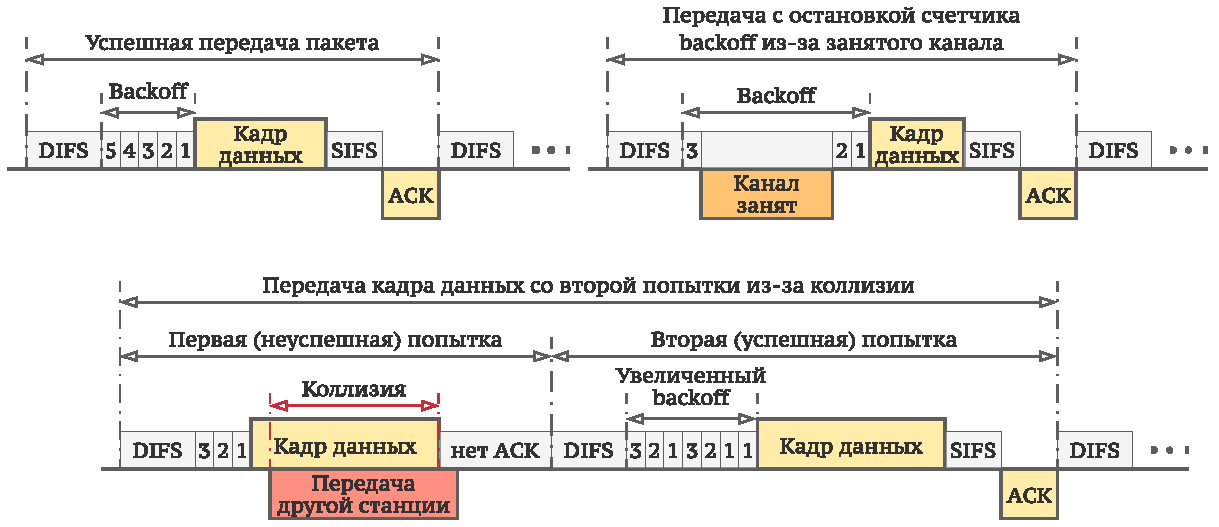
\includegraphics[width=0.9\textwidth]{chapter1/ch1_dcf}
	\caption{Организация доступа к каналу при использовании простейшей версии механизма DCF}
	\label{fig:ch1_dcf}
\end{figure}

В действительности, механизм DCF имеет ряд дополнительных возможностей, позволяющих увеличить эффективность передачи. Во-первых, если передаваемые данные имеют достаточно большой размер, перед их передачей станция может отправить кадр RTS (Request to Send), в котором передается ожидаемое время занятости канала. В ответ на RTS получатель передает CTS (Clear to Send), которым подтверждает готовность вести прием. Этот механизм позволяет решить проблему скрытых станций. Во-вторых, после успешной передачи станция может начать отсчет backoff (так называемый post-backoff) и, если новый пакет придет от сетевого уровня до того, как отсчет закончится, ему потребуется ждать передачи меньше времени. Количество попыток передачи пакета ограничено, и при его достижении пакет, вообще говоря, отбрасывается как недоставленный. Стоит также отметить, что при передаче больших пакетов может использоваться дефрагментация, и отдельные фрагменты могут передаваться без дополнительных отсчетов backoff. В диссертационной работе эти механизмы не учитываются, однако в дальнейшем их можно учесть для повышения точности моделирования. Что касается post-backoff и передачи группы кадров получившей доступ к каналу станцией (EDCF), для их адекватного учета нужно использовать более сложные методы описания времени передачи, например "--- марковские процессы обслуживания (MSP).


%%% --------------------------------------------
\subsection{Обзор исследований производительности беспроводных каналов связи}\label{sec:ch1_wifi_observe}
%%% --------------------------------------------

Из всех характеристик беспроводных каналов, в диссертационном исследовании основной интерес представляет время, необходимое для передачи одного сообщения. Для оценки длительности передачи сообщений, а также для оценки пропускной способности канала часто используются марковские или полумарковские случайные процессы. В таких моделях состояние случайного процесса описывает состояние канала (например, <<канал занят, ждать ещё два слота>> или <<ведётся передача>>), и производится оценка либо доли времени, которое процесс находится в определенных состояниях, либо времени, нужного для попадания в некоторое состояние. Использованию марковских и полумарковских процессов для анализа производительности беспроводных сетей на основе CSMA/CA посвящено большое количество работ, одной из ключевых является статья Bianchi \cite{Bianchi2000}, в которой была предложена марковская цепь, моделирующая работу станции сети IEEE 802.11 под управлением механизма доступа DCF. Состояния цепи соответствуют слотам ожидания backoff и попыткам передачи. Важным допущением модели является постоянство условной вероятности коллизии при передаче, а также насыщенный режим работы. С помощью предложенной цепи рассчитывается пропускная способность сети в насыщенном режиме. Полумарковские процессы также часто используются для описания работы беспроводной сети. Например, в работе \cite{Lauwens2010} предложен полумарковский процесс, моделирующий работу канального уровня сети IEEE 802.15.4-2006. Вместе с полумарковским процессом рассматривается процесс восстановления, моделирующий физический уровень. Предложенная авторами аналитическая модель используется для оценки пропускной способности сети, а кроме этого "--- оценки интервалов между успешными передачами и распределения длительности ожидания в backoff.

Так как DCF является наиболее базовым механизмом доступа, используемым в сетях IEEE 802.11, анализ длительности передачи пакетов в каналах DCF подробно рассматривался в большом числе работ (например, \cite{Chat2002, Banchs2006, Sakurai2007, Vardakas2007, Dong2008, Hung2007, Tickoo2008, Felemban2011, Haghani2011, Dai2013, Issar2005}). Отметим, что многие из этих работ основаны на марковском процессе, описанном Bianchi \cite{Bianchi2000}. Так, Chatzimisios и соавторы в работе \cite{Chat2002} описывают простейшую модель для расчета среднего времени передачи пакетов, основанную на модели Bianchi, предполагая ограниченное количество попыток передачи. В работе \cite{Banchs2006} также представлена аналитическая модель для вычисления задержек в передаче пакетов в ad-hoc сети IEEE 802.11 под управлением DCF в нагруженном режиме; помимо самой задержки, авторы анализируют сценарии использования сети для передачи голосовых и обычных данных. Авторы \cite{Sakurai2007} рассматривают работу ad-hoc сети в насыщенном режиме под управлением механизма DCF, получают аналитические выражения для математического ожидания и дисперсии времени обслуживания пакета, учитывая при этом ограниченное количество попыток передачи. Авторы также дают выражение для производящей функции моментов времни передачи пакета и исследуют функцию распределения этого времени. В работе \cite{Vardakas2007} рассматривается задержка, учитывающая также нахождение пакета в очереди. В работе \cite{Dong2008} Dong и соавторы изучают работу ad-hoc сети в ненасыщенном режиме, предполагая экспоненциальное распределение интервалов времени между поступлениями пакетов, и, помимо анализа времени обслуживания на отдельных узлах, рассматривают задержку при передаче по многошаговым маршрутам, учитывая наличие скрытых станций. Также проблеме измерения времени передачи при наличии скрытых станций посвящена работа \cite{Hung2007}. В работе \cite{Tickoo2008} представлен не только делательный анализ времени передачи пакетов в ad-hoc сети в ненагруженном режиме, но и рассматривается случай передачи группы пакетов при использовании механизма EDCA из IEEE 802.11e. Felemban и Ekici в работе \cite{Felemban2011} анализируют время передачи пакетов в одношаговых ad-hoc сетях, уточняя модель Bianchi за счет введения дополнительных марковских цепей в backoff-состояниях; ими также рассматривается случай ненасыщенной работы сети (при этом предполагается, что пакеты поступают в пуассоновском потоке). Также ненагруженный режим рассматривается в работе \cite{Duffy2005}. Еще один детальный анализ производительности ad-hoc сетей, включая длительности передачи пакетов, представлен в работе \cite{Dai2013}. Следует также выделить работу \cite{Issar2005}, в которой время передачи пакета описано как PH-распределение.

%Отметим, что целью нашей работы является не столько моделирование времени передачи пакетов на отдельных каналах, сколько использование полученных моделей времени для использования в составе тандемных сетей массового обслуживания типа $MAP/PH/1/N \rightarrow \dots \rightarrow \bullet/PH/1/N$ для оценки характеристик беспроводных сетей с линейной топологией. Хотя далее мы предлагаем использовать простую полумарковскую модель для анализа времени передачи пакетов в сети, работающей в насыщенном режиме (и показываем, что в некоторых случаях это дает хорошую оценку), для уточнения результатов можно использовать оценки времени передачи из приведенных выше работ, в особенности это касается ненасыщенного режима работы сети.

Ряд исследований рассматривают и сравнивают различные схемы доступа, используемые в сетях IEEE 802.11. Можно выделить работу \cite{Gao2005}, в которой рассматриваются режимы доступа EDCA и HCF, определенные в стандарте IEEE 802.11е и обсуждается их применимость к передаче данных мультимедиа. Также можно выделить работу \cite{Charfi2012}, авторы которой приводят описание как основных методов доступа DCF, PCF, EDCA, HCCA, так и дополнения, вводимые расширениями IEEE 802.11ac и IEEE 802.11ad (следует отметить, что статья вышла в 2012 году, когда расширения IEEE 802.11ac и IEEE 802.11ad еще находились на стадии разработки). Анализ производительности методов доступа EDCA \cite{Engelstad2006, Hazra2011, Kong2004, Liu2007, Inan2009, Misic2012, YanfengZhu2006} и HCCA \cite{Harsha2006, Ghazizadeh2009, Rashd2006}, введенных в стандарте IEEE 802.11e, широко рассмотрен в литературе. В работе \cite{Engelstad2006} с помощью аппарата марковских цепей и систем M/G/1 анализируется пропускная способность канала связи при использовании метода EDCA, а также полная задержка пакетов, включая время ожидания в очереди. В работе \cite{Hazra2011} также предлагается использовать марковскую цепь для анализа производительности, а предложенная авторами модель учитывает блочные подтверждения и агрегацию кадров. Еще один пример марковской цепи, используемой для анализа EDCA, приведен в работе \cite{Kong2004}. Авторы работы \cite{Liu2007} анализируют задержки и пропускные способности каналов под управлением EDCA при передачи разных типов трафика. В работе \cite{Misic2012} приводится большая аналитическая модель, позволяющая анализировать производительность EDCA в ненагруженном режиме. Следует также отметить работу \cite{YanfengZhu2006}, в которой авторы предлагают для анализа DCF и EDCA использовать модель PH/PH/1. В работе \cite{Harsha2006} авторы предлагают модель для анализа производительности канала связи при передаче голоса с использованием метода доступа HCCA и данных с использованием метода доступа EDCA. В работе \cite{Ghazizadeh2009} предлагается модель массового обслуживания MAP/PH/1 с приоритетами и периодами отдыха для анализа метода доступа HCCA.  Авторы работы \cite{Rashd2006} также используют марковскую систему массового обслуживания с отдыхами для моделирования HCCA.

В более поздних работах исследуются нововведения в протоколы MAC-уровня, появившихся в дополнениях IEEE 802.11ac и IEEE 802.11ad. Так, в работе \cite{Khan2017} анализируется производительность канала IEEE 802.11ac с использованием MIMO, учитывающая особенности как канального, так и физического уровня; нужно отметить, что в качестве модели канала используется, фактически, модель Bianchi \cite{Bianchi2000}. В работе \cite{Ong2011} приводится сравнение производительности IEEE 802.11n и IEEE 802.11ac, акцент сделан на исследовании механизмов агрегации кадров. Авторы работы \cite{Chandra2017} предлагают марковскую модель для анализа производительности миллиметровых каналов IEEE 802.11ad, учитывая такие особенности канала, как разделение пространства вокруг базовой станции на сектора.


%%%%%%%%%%%%%%%%%%%%%%%%%%%%%%%%%%%%%%%%%%%%%%%%%%%%%%%%%%%%%%%%%%%%%%%%%%%%%%%%
\section{Методы исследования задержек в многошаговых беспроводных сетей}\label{sec:ch1_qs}
%%%%%%%%%%%%%%%%%%%%%%%%%%%%%%%%%%%%%%%%%%%%%%%%%%%%%%%%%%%%%%%%%%%%%%%%%%%%%%%%

Способы получения оценок задержек и пропускной способности сетей можно разбить на три группы: стендовые, имитационные и аналитические. Стендовые измерения проводятся на реальной сети или ее макете. Эти измерения наиболее точные, но очень ресурсозатратные, трудоемкие и не всегда осуществимые. Имитационные измерения проводятся с помощью разчлиных систем имитационного моделирования, в которых сеть моделируется с помощью набора алгоритмов. Обычно эти алгоритмы воспроизводят работу моделируемых протоколов с высокой точностью. Наиболее популярные открытые системы имитационного моделирования NS-3 и OMNeT++ содержат реализации большинства распространенных сетевых протоколов, в том числе IEEE 802.11 (WiFi) и IEEE 802.3 (Ethernet). Преимущество имитационного моделирования "--- высокая точность, сопоставимая с измерением на стенде, и возможность получить множество различных характеристик с одного запуска. Главный недостаток "--- высокая вычислительная сложность. Наконец, аналитические методы позволяют найти оценки исследуемых параметров с помощью математических моделей. Чаще всего эти математические модели абстрагируются от всего, что не связано непосредственно с исследуемыми характеристиками. В зависимости от конкретной модели, оценки возможно получить гораздо быстрее, чем с помощью имитационного моделирования. Однако, из-за высокой степени абстракции, ошибки могут быть достаточно высокими.

Для аналитической оценки времени, которое требуется пакету для прохождения по сети, чаще всего используется аппарат теории массового обслуживания. В рамках этого подхода интервалы между поступающими в сеть пакетами и времена передачи пакетов в каналах связи моделируются случайными распределениями, а память в интерфейсах коммутаторов "--- очередями, в которых пакеты ожидают начала обслуживания. От того, насколько удачно выбраны случайные распределения, зависит точность полученных результатов. Помимо оценки задержек, модели массового обслуживания позволяют оценить необходимую емкость очередей и оценить вероятность потери пакетов из-за их переполнений.

Выбор модели входящего потока, то есть распределений интервалов между поступлениями пакетов в сеть, зависит от передаваемого сетью трафика. В общем случае, сетевой трафик является коррелированным \cite{Heyman2003, Klemm2003}. Для представления такого трафика можно использовать модель марковских коррелированных потоков (Markovian Arrival Process, MAP).

Время передачи пакета в канале связи складывается из ожидания начала передачи, непосредственно времени передачи пакета, а также времени ожидания и получения подтверждения доставки (если протокол реализует подтверждения). Если канал ненадежен и в нем возможны потери, то приходится также учитывать неуспешные попытки передачи. Таким образом, выбор модели распределения времени обслуживания зависит от схемы доступа, которая используется в канале связи, окружения и размеров передаваемых пакетов. Для моделирования времени передачи можно использовать распределения фазового типа (Phase-Type, PH), или более общую коррелированную модель "--- марковские процессы обслуживания (Markovian Service Process, MSP). В диссертационном исследовании будем использовать PH-распределения, но многие выводы можно обощить и на случай MSP.


%%% --------------------------------------------
\subsection{Открытые сети массового обслуживания с марковскими потоками заявок и обслуживанием фазового типа}
\label{sec:ch1_qs_map_ph}
%%% --------------------------------------------

Для анализа характеристик многошаговых телекоммуникационных сетей используются модели открытых тандемных сетей массового обслуживания \cite{Vishnevskii2017, VishnevskyDudin2018}. Такие модели состоят из обслуживающих устройств с очередями (узлов), последовательно соединенных друг с другом (см. рис.~\ref{fig:ch1_qs}). Для простоты, будем считать, что весь внешний трафик поступает на первый узел, и передается последовательно через все промежуточные узлы. В более общем случае в сети может присутствовать кросс-трафик, то есть поступления пакетов снаружи на промежуточные узлы, а маршрутизация может быть сложнее, например "--- пакеты могут передаваться вперед через несколько узлов или даже назад, образуя циклы.

\begin{figure}[ht]
  \centering
   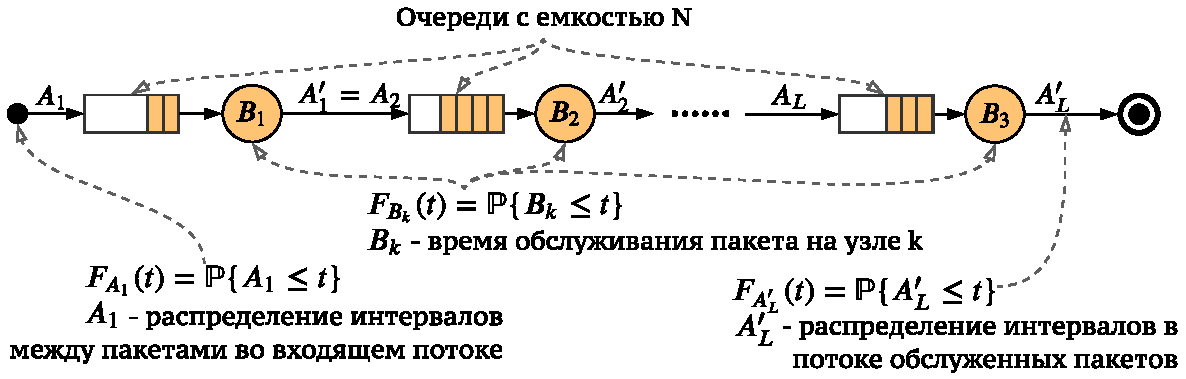
\includegraphics [scale=0.75] {chapter1/ch1_qs}
  \caption{Открытая сеть массового обслуживания с линейной топологией}
  \label{fig:ch1_qs}
\end{figure}

Если в качестве распределения времени обслуживания использовать PH-распределения, а в качестве модели входящего трафика "--- MAP-потоки, то выходящий поток обслуженных пакетов из узла MAP/PH/1/N будет также MAP \cite{Dudin2000}. Благодаря этому свойству рассчитывать характеристики открытой сети с линейной топологией с узлами MAP/PH/1/N можно с помощью простой итерационной процедуры, которая будет рассматриваться в главе 4.

PH-распределения являются обощением экспоненциальных распределений и могут использоваться для приближения любого непрерывного распределения на множестве неотрицательных чисел (см., например, \cite{Johnson1989}). Случайная величина $B$ имеет PH-распределение, если ее можно выразить как время, проведенное в некоторой непрерывной цепи Маркова с генератором $\widetilde{S}$, до попадания в поглощающее состояние. PH-распределение задается квадратной матрицей $S \in \mathbb{R}^{V \times V}$ и вектором начального распределения $\overline{\tau} \in \mathbb{R}^V$, для которых должно выполняться:

\begin{equation}\label{eq:ch1_ph_def}
  \begin{aligned}
    &\tilde{S} = \begin{bmatrix}
      S  & -S\mathbf{1} \\
      \mathbf{0} &  0
    \end{bmatrix} \mbox{"--- инфинитезимальная матрица,}\\
    &\forall i = \overline{1,V}: \: 0 \leq \tau_i \leq 1, \qquad
      \sum\limits_{i=1}^{V} \tau_i = 1.
  \end{aligned}
\end{equation}
Функция распределения случайной величины $B \sim PH(S, \overline{\tau})$ имеет вид $F_B(x) = \mathbb{P}\{B < x\} = 1 - \overline{\tau} e^{Sx} \mathbf{1}$~\cite{Buchholz2014}.

Марковские входные потоки (MAP) были впервые описаны в работах Neuts \cite{Neuts1979}. В ряде последующих исследований~\cite{Heyman2003, Klemm2003, Scott2003} было показано, что использование MAP-потоков позволяет достаточно точно моделировать сетевой трафик. MAP-поток $A \sim MAP(D_{0},D_{1})$ является обобщением PH-распределений и позволяет учесть корреляцию между значениями с лагом $k$. Распределения интервалов между событиями в MAP-потоке описываются PH-распределениями с одинаковыми матрицами $S \equiv D_0$, но меняющимися начальными векторами $\overline{\tau}_i$, зависящими от того, в каком состоянии находился процесс при появлении предыдущего события. MAP-поток определяется с помощью двух матриц, сумма которых $D=D_{0}+D_{1} \in \mathbb{R}^{W \times W}$ "--- инфинитезимальный генератор марковской цепи с непрерывным временем, управляющей переходами между состояниями процесса. Матрицы удовлетворяют ограничениям:

\begin{equation}\label{eq:ch1_map_def}
  \begin{aligned}
    &\forall i: \sum\limits_{j=1} \{D\}_{ij} = 0, \quad
      \forall i \neq j: \{D\}_{ij} \geq 0, \quad
      \forall i: \{D\}_{ii} \leq 0,\\
    &\forall i, j: \{D_{1}\}_{ij} \geq 0,\quad
      \forall i \neq j: \{D_{0}\}_{ij} \geq 0, \quad
      \forall i: \{D_{0}\}_{ii} \leq 0.
  \end{aligned}
\end{equation}

Более подробно свойства MAP-потоков и PH-распределений, которые потребуются для расчета характеристик тандемных сетей массового обслуживания, будут описаны в главе 4.

Помимо MAP-потока, иногда рассматриваются его обобщения на случай группового поступления пакетов (Batch MAP, BMAP)~\cite{Lucantoni1993, Dudin2000, VishnevskyDudin2018} или поступлений пакетов с разными приоритетами (Marked Markovian Arrival Process, MMAP)~\cite{HE2001, VanHoudt2012, Buchholz2010, Klimenok2020}. В обоих случаях вместо двух матриц $D_0$ и $D_1$ рассматривается набор матриц $D_i, i = \overline{0,K}$, где матрицы $D_i$ при $i > 0$ соответствуют поступлению группы $i$ пакетов (для BMAP) или пакета $i$-го типа (для MMAP).

Одна из основных проблем, возникающих при получении численных характеристик сетей массового обслуживания с узлами MAP/PH/1/N "--- экспоненциальный рост пространства состояний, из-за которого точный расчет возможен только для задач небольшой размерности. В связи с этим, для практического использования этой модели важно найти эффективные методы расчета характеристик тандемной сети массового обслуживания.

Исследованиям сетей массового обслуживания с MAP-потоками и PH-распределениями времени обслуживания посвящено множество работ. Например, в~\cite{Strelen1998, Henderson1990, Strelen1997, Strelen1997a} предлагаются методы вычисления характеристик сетей массового обслуживания на основе методов декомпозиции и представления искомых характеристик в форме произведений. В ряде работ акцент сделан на тандемных сетях массового обслуживания и изучениии их характеристик \cite{Kim2018, Kim2012, Kim2007, Buchholz2006}, а также исследованию выходных потоков из систем массового обслуживания с марковскими входными потоками \cite{Bean1998, Lian2011}.

%%% --------------------------------------------
\subsection{Методы восстановления PH-распределений и MAP-потоков}\label{sec:ch1_qs_ph_fitting}
%%% --------------------------------------------

Методы поиска PH-распределений и MAP-потоков в диссертационном исследовании будут применяться для решения двух задач: для поиска распределений, моделирующих время передачи пакетов в каналах связи, и для поиска MAP-потоков меньшей размерности, аппроксимирующих потоки обслуженных пакетов на выходе из очередного узла тандемной сети.

Для поиска PH-распределения или MAP-потока можно использовать два подхода: принцип максимального правдоподобия и метод моментов. В первом случае необходима выборка значений распределения, на которой максимизируется функция правдоподобия. Существует ряд реализаций, основанных на методе максимизации ожидания (EM-процедуре) для MAP-потоков \cite{Horvath2013,Ephraim2009,Buchholz2003,Okamura2009} и PH-распределений \cite{Asmussen1996,Bobbio1992,Thummler2005,Okamura2013,Okamura2011,ElAbdouniKhayari2003}. Главное ограничение метода "--- высокая вычислительная сложность, что ограничивает его использование в итерационных алгоритмах, где его необходимо применять многократно. Из-за этого в диссертационном исследовании этот подход не будет использоваться, хотя он оказывается достаточно удобным при поиске MAP-потоков и PH-распределений при моделировании реальных входящих данных, полученных, например, из сетевого дампа.

Второй подход основан на методе моментов. Он применяется как для PH-распределений \cite{Osogami2006,Bobbio2005,Johnson1989,Telek2003,Horvath2013,VandenBosch2000,Horvath2007,Schmickler1992}, так и для MAP-потоков \cite{TelekHorvath2007,Bodrog2010,Bodrog2008,Horvath2005,Schmickler1992,Casale2010}. В первом случае PH-распределение строится по известным значениям первых моментов $m_1, m_2, \dots m_K$ случайной величины, во втором также могут учитываться значения коэффициентов корреляции $l$-го порядка (с лагом $l$) $\rho_1, \rho_2, \dots, \rho_L$.

Сложность применения метода моментов заключается в том, что точные области существования PH-распределений и MAP-потоков заданной размерности $W$, то есть множество значений моментов $m_1, m_2, \dots m_K$ и коэффициентов корреляции $\rho_1, \rho_2, \dots, \rho_L$ при сколь угодно больших $K$ и $L$, для которых существует PH-распределение или MAP-поток размерности $W$, имеют сложный вид~\cite{Bobbio2005,Osogami2006,TelekHorvath2007,Bodrog2008,Bodrog2010}. Другими словами, при известных значениях моментов и коэффициентов корреляции сложно не только найти PH-распределение или MAP-поток минимально возможного порядка, но и даже определить этот порядок. При этом, хорошо известны грубые оценки, связывающие размерность и значения моментов. Например, в работе \cite{Aldous1987} доказано, что среди всех PH-распределений заданного размера наименьшее значение коэффициента вариации достигается на распределении Эрланга, что позволяет грубо оценить снизу размерность искомого PH-распределения при известных первом и втором моменте. Есть методы, позволяющие находить распределения малого порядка, но не для любых наборов значений моментов. Например, в работе \cite{Telek2003} исследуется область существования ациклических PH-распределений второго порядка APH(2), а в работе \cite{Bodrog2010} Bodrog и соавторы исследуют область существования MAP-потоков второго порядка. Telek и Horvath \cite{TelekHorvath2007} описывают минимальные формы PH-распределений и MAP-потоков (марковская, жорданова и прочие формы), а также преобразования между ними. Авторы предлагают алгоритм оптимизации матриц $D_0$ и $D_1$, позволяющий минимизировать целевую функцию, зависящую от $B^{-1}D_{0}B$ и $B^{-1}D_{1}B$ посредством поиска матрицы преобразования $B$. Предложенный метод позволяет улучшить MAP-поток, который был получен любым другим методом.

Если ограничения на порядок существенны, то в общем случае приходится искать такой MAP-поток $X \sim MAP(D_0, D_1)$ (PH-распределение $Y \sim PH(S, \overline{\tau})$), чтобы выполнялись ограничения \eqref{eq:ch1_map_def} (для PH-распределения "--- \eqref{eq:ch1_ph_def}), и достигался минимум функции ошибки при заданных весах $\overline{w}$:

$$
  \begin{aligned}
    \mathcal{L}_{\text{MAP}}(X; \overline{m}, \overline{\rho}, \overline{w}) &=
      \sum\limits_{k=1}^K w_k (m'_k - m_k)^2 +
      \sum\limits_{l=1}^L w_{K+l} (\rho'_l - \rho_l)^2
      \rightarrow \text{min},\\
    \mathcal{L}_{\text{PH}}(Y; \overline{m}, \overline{w}) &=
      \sum\limits_{k=1}^K w_k (m'_k - m_k)^2
      \rightarrow \text{min}.
  \end{aligned}
$$
Здесь $m'_k$ "--- $k$-й момент MAP-потока $X$ или PH-распределения $Y$, а $\rho'_l$ "--- коэффициент корреляции $X$ с лагом $l$.

При поиске PH-распределений чаще всего накладываются ограничения на структуру матрицы $S$, то есть поиск ведется по некоторому подсемейству распределений. Есть реализации метода моментов \cite{Johnson1989, Bobbio2005, Horvath2007, Horvath2013}, которые позволяют находить распределения по произвольному набору моментов. В работе Johnson и Taafe \cite{Johnson1989} предлагают искать PH-распределения по заданным трем моментам в виде гиперэрланговского распределения с двумя цепочками Эрланга одинакового порядка. Bobbio и соавторы \cite{Bobbio2005} предлагают метод поиска ациклических PH-распределений APH(n) минимального порядка $n$ также по первым трем моментам; кроме того, авторы описывают границы значений первых трех моментов для распределений APH(n) при известном $n$. В работе \cite{Horvath2013} Horvath и соавторы предлагают метод поиска по произвольному числу первых моментов специального подкласса PH-распределений "--- обобщенных гиперэрланговских распределений. Метод позволяет находить множество допустимых PH-распределений, из которых можно выбрать наиболее подходящее по той или иной метрике. Casale и соавторы \cite{Casale2010} предлагают метод поиска MAP-потоков по первым трём моментам и коэффициентам корреляции как композиции MAP-потоков меньших размеров (метод композиции через кронекерово произведение, Kronecker Product Composition, KPC).

Если задача состоит в поиске MAP-потока $X'$ с теми же характеристиками, что и MAP-поток $X$, но имеющего меньший порядок, то можно использовать и другие подходы. Например, простой метод сокращений пространства состояний основан на идее о том, что некоторые состояния MAP-потока большой размерности избыточны, и их можно удалить. Этот метод применим для систем MAP/PH/1 и MAP/PH/1/N, в которых коэффициент загрузки достаточно мал. Например, авторы работы \cite{Horvath2010} рассматривают выходной поток (обслуженных пакетов) системы MAP/MAP/1 и предлагают удалять блоки матриц $D_0,\,D_1$, соответствующие числу пакетов в системе свыше заданного уровня $N$.

В диссертационной работе для поиска PH-распределений и MAP-потоков будет использоваться метод моментов, а именно "--- простой метод поиска PH-распределений по первым трем моментам в виде распределений гиперэрланга с двумя цепями одинаковых порядков, предложенный в работе Johnson и Taafe \cite{Johnson1989}. При поиске MAP-потока этот метод будет использоваться для расчета матрицы $D_0$, а поиск матрицы $D_1$ будет производиться отдельно по заданным коэффициентам корреляции, как предложено в работе Horvath и соавторов \cite{Horvath2005}. Как показали численные эксперименты, эта комбинация методов просто реализуется, работает достаточно хорошо и стабильно и позволяет находить распределения за короткое время, хотя порядки могут быть несколько больше, чем в альтернативных методах. Время работы особенно критично, так как в численном эксперименте требовалось рассчитать характеристики нескольких сотен сетей с узлами MAP/PH/1/N.



%%%%%%%%%%%%%%%%%%%%%%%%%%%%%%%%%%%%%%%%%%%%%%%%%%%%%%%%%%%%%%%%%%%%%%%%%%%%%%%%
\section{Методы построения распределённых систем радиочастотной идентификации}
%%%%%%%%%%%%%%%%%%%%%%%%%%%%%%%%%%%%%%%%%%%%%%%%%%%%%%%%%%%%%%%%%%%%%%%%%%%%%%%%

С момента появления технологии RFID ведутся исследования в области создания систем управления считывателями и промежуточного программного обеспечения (Middleware). Хороший обзор ранних подходов и практически реализованных систем приведен в работе Al-Jaroodi и соавторов \cite{Al-Jaroodi2009}, где они рассматривают общие требования к промежуточному программному обеспечению для RFID и анализируют семь различных систем с точки зрения надёжности, масштабируемости, балансировке нагрузки, возможности управления данными и безопасности. В более позднем обзоре Razzaque и соавторы \cite{Razzaque2016}, рассматривая RFID уже в качестве неотъемлемой части Интернета вещей (Internet of Things, IoT), расширяют список требований, предъявляемых к промежуточному программному обеспечению, рассматривая требования к программным интерфейсам, необходимость реализации программного обеспечения в рамках сервисно-ориентированной модели Software-as-a-Service (SaaS) и Everything-as-a-Service (XaaS).

Для подключения RFID-считывателей к системам управления используются стандартные протоколы, которые поддерживаются большинством производителей. Протокол Low Level Reader Protocol (LLRP) \cite{StdLlrp} определяет низкоуровневый интерфейс между считывателем и контроллером. Этот протокол позволяет выполнять произвольные операции доступа и инвентаризации, настраивать параметры радиоинтерфейса считывателя, получать данные о состоянии радиоканала и диагностические данные о работе считывателя. Протокол LLRP поддерживается большинством существующих считывателей. Стандарт определяет возможность работы протокола по каналам TLS. Помимо LLRP, организация EPCglobal опубликовала несколько стандартов \cite{StdRm, StdDci, StdAle1, StdAle2}, которые можно использовать при разработке считывателя и системы управления. Стандарт <<Reader Management 1.0.1 (RM)>> \cite{StdRm} определяет модель системы и MIB (Management Information Base) для сбора данных о состоянии работы считывателя через протокол SNMP. Стандарт <<Discovery, Configuration, and Initialization (DCI) for Reader Operations>> \cite{StdDci} позволяет считывателю, контроллерам и LLRP-клиентам находить друг друга в сети, производить аутентификацию между контроллерами и считывателями, управлять работой считывателей, загружать новые образы программного обеспечения и выполнять прочие служебные функции. Стандарт <<Application Level Events (ALE) Standard>> \cite{StdAle1, StdAle2} описывает рекомендации по разработке промежуточного программного обеспечения. Кроме стандартов EPCglobal, существует спецификация интерфейса между считывателем и контроллером от альянса RAIN RFID \cite{StdRainRci}. Эта спецификация более высокоуровневая, по сравнению с LLRP. Она описывает основные действия, включая конфигурацию и получение статуса считывателя, настройки радиопротокола, доступ к меткам. Спецификация определяет сообщения, передаваемые между считывателем и конроллером, в формате JSON.

В целом ряде ранних исследовательских работ \cite{Hoag2006,Yu2009,XiuLi2012,Koutsoubelias2007,Abad2012,Chien-ChangHsu2008,Floerkemeier2007} рассматриваются детали архитектуры и подходов к построению промежуточного программного обеспечения, причем материал некотрых из них и на сегодняшний день представляет интерес. Например, Hoag и Thompson в работе \cite{Hoag2006} выделяют два уровня архитектуры: уровень агентов и уровень RFID-приложений. Предложенная архитектура допускает подключение различного оборудования (считыватели, принтеры меток, базы данных и пр.) через специальных модулей--агентов, использующих для обмена сообщениями унифицированный транспортный уровень, на котором реализуются как односторонние обмены сообщениями, так и многоадресные соединения для связи типа <<публикация--подписка>>. Архитектура системы на основе механизма подписок также рассматривается в работе Yu и Lai~\cite{Yu2009}. В работе~\cite{XiuLi2012} описывается двухуровневая архитектура промежуточного программного обеспечения RFID с фильтрацией и агрегацией данных, а в работе~\cite{Koutsoubelias2007} предлагается построение промежуточного программного обеспечения с использованим адаптеров, предоставляющих унифицированный интерфейс для подключения считывателей. Авторы \cite{Chien-ChangHsu2008} предлагают модель системы управления считывателями и промежуточным программным обеспеченим, направленную на повышение отказоустойчивости. Наконец, ещё один ранний проект открытого промежуточного программного обеспечения для RFID (Accada) был предложен в работе Floerkemeier и соавторов \cite{Floerkemeier2007}. В нем авторы поднимают ряд проблем, от различия между требованиями пользователей вплоть до многолучевого распространения сигналов, и предлагают оригинальные решения, например "--- использование виртуальной памяти для отложенной записи данных на метки или механизм прогнозирования длительности нахождения меток в области чтения.

В более поздних исследованиях разработчики систем управления и промежуточного программного обеспечения рассматривают RFID в более широком контексте интернета вещей (IoT). В работе \cite{Santos2019} предложена пятиуровневая модель, в которой данные со считывателя поступают в облако и обрабатываются при помощи различных микросервисов. Aazam и Huh в работе \cite{Aazam2016} рассматривают системы управления и взаимодействия с устройствами (в частности, с RFID-считывателями и метками) в контексте интернета вещей (IoT), интернета всего (Internet of Everything, IoE) и туманных вычислений (Fog Computing). Например, в работе \cite{Schreiber2012} Schreiber с соавторами предлагают архитектуру промежуточного программного обеспечения, позволяющего единообразно работать с RFID-считывателями и сенсорами. Помимо детального описания архитектуры, авторы также предлагают SQL-подобный язык, позволяющий пользователю строить запросы к системе, не вдаваясь в специфику того ли иного устройства. В более ранней работе \cite{Cho2007} Cho и соавторы рассматривают распределенную систему, позволяющую не просто идентифицировать объекты, но связывать данные о них с показателями сенсоров.

Хотя в большинстве работ промежуточное программное обеспечение включает в себя функции как для получения и обработки данных о прочитанных метках, так и функции управления и мониторинга состояния считывтелей, некоторые авторы допускают их разнесение. Например, Kamoun в работе \cite{Kamoun2009} предполагает, что системы управления считывателями лучше не рассматривать в контексте промежуточного программного обеспечения, оставив последнему функции по работе с данными. В работе \cite{JongyoungLee2006} производится анализ и выбор метрик производительности промежуточного программного обеспечения для RFID. Авторы рассматривают в качестве метрик зависимости загрузки системы (использование процессоров и памяти) и времени отклика на запросы клиентов от числа подключенных считывателей, числа подключенных приложений (клиентов), а также количества читаемых каждым считывателем меток. Также авторы описывают дизайн системы анализа производительности промежуточного программного обеспечения для RFID и приводят краткое описание собственной реализации.

Многие исследования направлены на разработку программного обеспечения для специализированных применений RFID. Например, в работе \cite{Henao2019} описывается архитектура информационной системы, в которой один терминал (клиент) подключается ко множеству считывателей (серверов), для применения на автомобильном заводе. Статья \cite{Figueroa2019} посвящена описанию системы отслеживания местонахождения людей с помощью имплантированных RFID-чипов под кожу. В работе \cite{Zhang2018} описана информационная система для управления библиотечным фондом с использованием RFID, авторы \cite{Li2010} описывают архитектуру и опыт реализации RFID-системы на фабрике по выпуску одежды, а в работе \cite{Shah2016} предлагается использовать RFID для систем обеспечения безопасности перевозки школьников в автобусах. В статье \cite{Chamekh2017} рассматривается использование RFID в области фармацевтики для контроля за качеством лекарств и отслеживанием контрафакта. Работы \cite{Rouchdi2018,Baskoro2018} посвящены системам отслеживания багажа в аэропортах с помощью RFID.

Помимо технической стороны разработки информационных систем с использованием RFID, есть ряд вопросов этики и безопасности, поскольку данные на метках находятся в тесной связи с людьми и бизнесом. Хорошую подборку и анализ как преимуществ внедрения RFID, так и проблем, связанных с этим (в частности, кражей данных и отношением людей к сбору данных о себе), можно найти в ранней работе \cite{Thompson2007}. В работе \cite{Figueroa2019} предлагается использовать блокчейн для распределенного контроля доступа к меткам. Бельский и соавторы \cite{Belsky2021} исследуют безопасность систем RFID и приводят описание моделей угроз. Авторы работы \cite{Bashir2011} описывают требования к распределенной системе управления мобильными RFID-считывателями, уделяя особое внимание вопросам безопасности. Также стоит выделить работу Fouladgar и Afifi \cite{Fouladgar2007}, в которой они предлагают безопасный протокол делегирования из доверенной центральной информационной системы прав на идентификацию меток считывателям.





\section{Заключение}\label{sec:ch1_conclusion}

В главе была описана общая структура системы радиочастотной идентификации транспорта, разработке и исследованию которой посвящена диссертационная работа. Выделены ключевые компоненты системы: RFID считыватели, метки, телекоммуникационная сеть и центр обработки данных; для каждого из компонентов поставлены задачи, решаемые в диссертационном исследовании.

После постановки задач исследования, в главе были описаны технологии, используемые в распределенной системе радиочастотной идентификации, и математические методы, используемые для их исследования. По всем упомянутым технологиям и методам был приведен обзор литературы и актуальных научных исследований. Также в общих чертах были выделены отличия и новизна предложенных в диссертации методов и подходов от существующих в литературе.






%\section{Форматирование текста}\label{sec:ch1/sec1}
%
%Мы можем сделать \textbf{жирный текст} и \textit{курсив}.
%
%\section{Ссылки}\label{sec:ch1/sec2}
%
%Сошлёмся на библиографию.
%Одна ссылка: \cite[с.~54]{Sokolov}\cite[с.~36]{Gaidaenko}.
%Две ссылки: \cite{Sokolov,Gaidaenko}.
%Ссылка на собственные работы: \cite{vakbib1, confbib2}.
%Много ссылок: %\cite[с.~54]{Lermontov,Management,Borozda} % такой «фокус»
%%вызывает biblatex warning относительно опции sortcites, потому что неясно, к
%%какому источнику относится уточнение о страницах, а bibtex об этой проблеме
%%даже не предупреждает
%\cite{Lermontov, Management, Borozda, Marketing, Constitution, FamilyCode,
%Gost.7.0.53, Razumovski, Lagkueva, Pokrovski, Methodology, Berestova,
%Kriger}%
%\ifnumequal{\value{bibliosel}}{0}{% Примеры для bibtex8
%    \cite{Sirotko, Lukina, Encyclopedia, Nasirova}%
%}{% Примеры для biblatex через движок biber
%    \cite{Sirotko2, Lukina2, Encyclopedia2, Nasirova2}%
%}%
%.
%И~ещё немного ссылок:~\cite{Article,Book,Booklet,Conference,Inbook,Incollection,Manual,Mastersthesis,
%Misc,Phdthesis,Proceedings,Techreport,Unpublished}
%% Следует обратить внимание, что пробел после запятой внутри \cite{}
%% обрабатывается ожидаемо, а пробел перед запятой, может вызывать проблемы при
%% обработке ссылок.
%\cite{medvedev2006jelektronnye, CEAT:CEAT581, doi:10.1080/01932691.2010.513279,
%Gosele1999161,Li2007StressAnalysis, Shoji199895, test:eisner-sample,
%test:eisner-sample-shorted, AB_patent_Pomerantz_1968, iofis_patent1960}
%\ifnumequal{\value{bibliosel}}{0}{% Примеры для biblatex через движок biber
%    \cite{patent2h, patent3h, patent2}%
%}%
%.
%
%\ifnumequal{\value{bibliosel}}{0}{% Примеры для bibtex8
%Попытка реализовать несколько ссылок на конкретные страницы
%для \texttt{bibtex} реализации библиографии:
%[\citenum{Sokolov}, с.~54; \citenum{Gaidaenko}, с.~36].
%}{% Примеры для biblatex через движок biber
%Несколько источников (мультицитата):
%% Тут специально написано по-разному тире, для демонстрации, что
%% применение специальных тире в настоящий момент в biblatex приводит к непоказу
%% "с.".
%\cites[vii--x, 5, 7]{Sokolov}[v"--~x, 25, 526]{Gaidaenko}[vii--x, 5, 7]{Techreport},
%работает только в \texttt{biblatex} реализации библиографии.
%}%
%
%Ссылки на собственные работы:~\cite{vakbib1, confbib1}
%
%Сошлёмся на приложения: Приложение~\cref{app:A}, Приложение~\cref{app:B2}.
%
%Сошлёмся на формулу: формула~\cref{eq:equation1}.
%
%Сошлёмся на изображение: рисунок~\cref{fig:knuth}.
%
%Стандартной практикой является добавление к ссылкам префикса, характеризующего тип элемента.
%Это не является строгим требованием, но~позволяет лучше ориентироваться в документах большого размера.
%Например, для ссылок на~рисунки используется префикс \textit{fig},
%для ссылки на~таблицу "--- \textit{tab}.
%
%В таблице \cref{tab:tab_pref} приложения~\cref{app:B4} приведён список рекомендуемых
%к использованию стандартных префиксов.
%
%\section{Формулы}\label{sec:ch1/sec3}
%
%Благодаря пакету \textit{icomma}, \LaTeX~одинаково хорошо воспринимает
%в~качестве десятичного разделителя и запятую (\(3,1415\)), и точку (\(3.1415\)).
%
%\subsection{Ненумерованные одиночные формулы}\label{subsec:ch1/sec3/sub1}
%
%Вот так может выглядеть формула, которую необходимо вставить в~строку
%по~тексту: \(x \approx \sin x\) при \(x \to 0\).
%
%А вот так выглядит ненумерованная отдельностоящая формула c подстрочными
%и надстрочными индексами:
%\[
%(x_1+x_2)^2 = x_1^2 + 2 x_1 x_2 + x_2^2
%\]
%
%Формула с неопределенным интегралом:
%\[
%\int f(\alpha+x)=\sum\beta
%\]
%
%При использовании дробей формулы могут получаться очень высокие:
%\[
%  \frac{1}{\sqrt{2}+
%  \displaystyle\frac{1}{\sqrt{2}+
%  \displaystyle\frac{1}{\sqrt{2}+\cdots}}}
%\]
%
%В формулах можно использовать греческие буквы:
%%Все \original... команды заранее, ради этого примера, определены в Dissertation\userstyles.tex
%\[
%\alpha\beta\gamma\delta\originalepsilon\epsilon\zeta\eta\theta%
%\vartheta\iota\kappa\varkappa\lambda\mu\nu\xi\pi\varpi\rho\varrho%
%\sigma\varsigma\tau\upsilon\originalphi\phi\chi\psi\omega\Gamma\Delta%
%\Theta\Lambda\Xi\Pi\Sigma\Upsilon\Phi\Psi\Omega
%\]
%\[%https://texfaq.org/FAQ-boldgreek
%\boldsymbol{\alpha\beta\gamma\delta\originalepsilon\epsilon\zeta\eta%
%\theta\vartheta\iota\kappa\varkappa\lambda\mu\nu\xi\pi\varpi\rho%
%\varrho\sigma\varsigma\tau\upsilon\originalphi\phi\chi\psi\omega\Gamma%
%\Delta\Theta\Lambda\Xi\Pi\Sigma\Upsilon\Phi\Psi\Omega}
%\]
%
%Для добавления формул можно использовать пары \verb+$+\dots\verb+$+ и \verb+$$+\dots\verb+$$+,
%но~они считаются устаревшими.
%Лучше использовать их функциональные аналоги \verb+\(+\dots\verb+\)+ и \verb+\[+\dots\verb+\]+.
%
%\subsection{Ненумерованные многострочные формулы}\label{subsec:ch1/sec3/sub2}
%
%Вот так можно написать две формулы, не нумеруя их, чтобы знаки <<равно>> были
%строго друг под другом:
%\begin{align}
%  f_W & =  \min \left( 1, \max \left( 0, \frac{W_{soil} / W_{max}}{W_{crit}} \right)  \right), \nonumber \\
%  f_T & =  \min \left( 1, \max \left( 0, \frac{T_s / T_{melt}}{T_{crit}} \right)  \right), \nonumber
%\end{align}
%
%Выровнять систему ещё и по переменной \( x \) можно, используя окружение
%\verb|alignedat| из пакета \verb|amsmath|. Вот так:
%\[
%    |x| = \left\{
%    \begin{alignedat}{2}
%        &&x, \quad &\text{eсли } x\geqslant 0 \\
%        &-&x, \quad & \text{eсли } x<0
%    \end{alignedat}
%    \right.
%\]
%Здесь первый амперсанд (в исходном \LaTeX\ описании формулы) означает
%выравнивание по~левому краю, второй "--- по~\( x \), а~третий "--- по~слову
%<<если>>. Команда \verb|\quad| делает большой горизонтальный пробел.
%
%Ещё вариант:
%\[
%    |x|=
%    \begin{cases}
%    \phantom{-}x, \text{если } x \geqslant 0 \\
%    -x, \text{если } x<0
%    \end{cases}
%\]
%
%Кроме того, для  нумерованных формул \verb|alignedat| делает вертикальное
%выравнивание номера формулы по центру формулы. Например, выравнивание
%компонент вектора:
%\begin{equation}
%\label{eq:2p3}
%\begin{alignedat}{2}
%{\mathbf{N}}_{o1n}^{(j)} = \,{\sin} \phi\,n\!\left(n+1\right)
%         {\sin}\theta\,
%         \pi_n\!\left({\cos} \theta\right)
%         \frac{
%               z_n^{(j)}\!\left( \rho \right)
%              }{\rho}\,
%           &{\boldsymbol{\hat{\mathrm e}}}_{r}\,+   \\
%+\,
%{\sin} \phi\,
%         \tau_n\!\left({\cos} \theta\right)
%         \frac{
%            \left[\rho z_n^{(j)}\!\left( \rho \right)\right]^{\prime}
%              }{\rho}\,
%            &{\boldsymbol{\hat{\mathrm e}}}_{\theta}\,+   \\
%+\,
%{\cos} \phi\,
%         \pi_n\!\left({\cos} \theta\right)
%         \frac{
%            \left[\rho z_n^{(j)}\!\left( \rho \right)\right]^{\prime}
%              }{\rho}\,
%            &{\boldsymbol{\hat{\mathrm e}}}_{\phi}\:.
%\end{alignedat}
%\end{equation}
%
%Ещё об отступах. Иногда для лучшей <<читаемости>> формул полезно
%немного исправить стандартные интервалы \LaTeX\ с учётом логической
%структуры самой формулы. Например в формуле~\cref{eq:2p3} добавлен
%небольшой отступ \verb+\,+ между основными сомножителями, ниже
%результат применения всех вариантов отступа:
%\begin{align*}
%\backslash! &\quad f(x) = x^2\! +3x\! +2 \\
%  \mbox{по-умолчанию} &\quad f(x) = x^2+3x+2 \\
%\backslash, &\quad f(x) = x^2\, +3x\, +2 \\
%\backslash{:} &\quad f(x) = x^2\: +3x\: +2 \\
%\backslash; &\quad f(x) = x^2\; +3x\; +2 \\
%\backslash \mbox{space} &\quad f(x) = x^2\ +3x\ +2 \\
%\backslash \mbox{quad} &\quad f(x) = x^2\quad +3x\quad +2 \\
%\backslash \mbox{qquad} &\quad f(x) = x^2\qquad +3x\qquad +2
%\end{align*}
%
%Можно использовать разные математические алфавиты:
%\begin{align}
%\mathcal{ABCDEFGHIJKLMNOPQRSTUVWXYZ} \nonumber \\
%\mathfrak{ABCDEFGHIJKLMNOPQRSTUVWXYZ} \nonumber \\
%\mathbb{ABCDEFGHIJKLMNOPQRSTUVWXYZ} \nonumber
%\end{align}
%
%Посмотрим на систему уравнений на примере аттрактора Лоренца:
%
%\[
%\left\{
%  \begin{array}{rl}
%    \dot x = & \sigma (y-x) \\
%    \dot y = & x (r - z) - y \\
%    \dot z = & xy - bz
%  \end{array}
%\right.
%\]
%
%А для вёрстки матриц удобно использовать многоточия:
%\[
%\left(
%  \begin{array}{ccc}
%    a_{11} & \ldots & a_{1n} \\
%    \vdots & \ddots & \vdots \\
%    a_{n1} & \ldots & a_{nn} \\
%  \end{array}
%\right)
%\]
%
%\subsection{Нумерованные формулы}\label{subsec:ch1/sec3/sub3}
%
%А вот так пишется нумерованная формула:
%\begin{equation}
%  \label{eq:equation1}
%  e = \lim_{n \to \infty} \left( 1+\frac{1}{n} \right) ^n
%\end{equation}
%
%Нумерованных формул может быть несколько:
%\begin{equation}
%  \label{eq:equation2}
%  \lim_{n \to \infty} \sum_{k=1}^n \frac{1}{k^2} = \frac{\pi^2}{6}
%\end{equation}
%
%Впоследствии на формулы~\cref{eq:equation1, eq:equation2} можно ссылаться.
%
%Сделать так, чтобы номер формулы стоял напротив средней строки, можно,
%используя окружение \verb|multlined| (пакет \verb|mathtools|) вместо
%\verb|multline| внутри окружения \verb|equation|. Вот так:
%\begin{equation} % \tag{S} % tag - вписывает свой текст
%  \label{eq:equation3}
%    \begin{multlined}
%        1+ 2+3+4+5+6+7+\dots + \\
%        + 50+51+52+53+54+55+56+57 + \dots + \\
%        + 96+97+98+99+100=5050
%    \end{multlined}
%\end{equation}
%
%Уравнения~\cref{eq:subeq_1,eq:subeq_2} демонстрируют возможности
%окружения \verb|\subequations|.
%\begin{subequations}
%    \label{eq:subeq_1}
%    \begin{gather}
%        y = x^2 + 1 \label{eq:subeq_1-1} \\
%        y = 2 x^2 - x + 1 \label{eq:subeq_1-2}
%    \end{gather}
%\end{subequations}
%Ссылки на отдельные уравнения~\cref{eq:subeq_1-1,eq:subeq_1-2,eq:subeq_2-1}.
%\begin{subequations}
%    \label{eq:subeq_2}
%    \begin{align}
%        y &= x^3 + x^2 + x + 1 \label{eq:subeq_2-1} \\
%        y &= x^2
%    \end{align}
%\end{subequations}
%
%\subsection{Форматирование чисел и размерностей величин}\label{sec:units}
%
%Числа форматируются при помощи команды \verb|\num|:
%\num{5,3};
%\num{2,3e8};
%\num{12345,67890};
%\num{2,6 d4};
%\num{1+-2i};
%\num{.3e45};
%\num[exponent-base=2]{5 e64};
%\num[exponent-base=2,exponent-to-prefix]{5 e64};
%\num{1.654 x 2.34 x 3.430}
%\num{1 2 x 3 / 4}.
%Для написания последовательности чисел можно использовать команды \verb|\numlist| и \verb|\numrange|:
%\numlist{10;30;50;70}; \numrange{10}{30}.
%Значения углов можно форматировать при помощи команды \verb|\ang|:
%\ang{2.67};
%\ang{30,3};
%\ang{-1;;};
%\ang{;-2;};
%\ang{;;-3};
%\ang{300;10;1}.
%
%Обратите внимание, что ГОСТ запрещает использование знака <<->> для обозначения отрицательных чисел
%за исключением формул, таблиц и~рисунков.
%Вместо него следует использовать слово <<минус>>.
%
%Размерности можно записывать при помощи команд \verb|\si| и \verb|\SI|:
%\si{\farad\squared\lumen\candela};
%\si{\joule\per\mole\per\kelvin};
%\si[per-mode = symbol-or-fraction]{\joule\per\mole\per\kelvin};
%\si{\metre\per\second\squared};
%\SI{0.10(5)}{\neper};
%\SI{1.2-3i e5}{\joule\per\mole\per\kelvin};
%\SIlist{1;2;3;4}{\tesla};
%\SIrange{50}{100}{\volt}.
%Список единиц измерений приведён в таблицах~\cref{tab:unit:base,
%tab:unit:derived,tab:unit:accepted,tab:unit:physical,tab:unit:other}.
%Приставки единиц приведены в~таблице~\cref{tab:unit:prefix}.
%
%С дополнительными опциями форматирования можно ознакомиться в~описании пакета \texttt{siunitx};
%изменить или добавить единицы измерений можно в~файле \texttt{siunitx.cfg}.
%
%\begin{table}
%    \centering
%    \captionsetup{justification=centering} % выравнивание подписи по-центру
%    \caption{Основные величины СИ}\label{tab:unit:base}
%    \begin{tabular}{llc}
%        \toprule
%        Название  & Команда                & Символ         \\
%        \midrule
%        Ампер     & \verb|\ampere| & \si{\ampere}   \\
%        Кандела   & \verb|\candela| & \si{\candela}  \\
%        Кельвин   & \verb|\kelvin| & \si{\kelvin}   \\
%        Килограмм & \verb|\kilogram| & \si{\kilogram} \\
%        Метр      & \verb|\metre| & \si{\metre}    \\
%        Моль      & \verb|\mole| & \si{\mole}     \\
%        Секунда   & \verb|\second| & \si{\second}   \\
%        \bottomrule
%    \end{tabular}
%\end{table}
%
%\begin{table}
%  \small
%  \centering
%  \begin{threeparttable}% выравнивание подписи по границам таблицы
%    \caption{Производные единицы СИ}\label{tab:unit:derived}
%    \begin{tabular}{llc|llc}
%        \toprule
%        Название       & Команда                 & Символ              & Название & Команда & Символ \\
%        \midrule
%        Беккерель      & \verb|\becquerel|  & \si{\becquerel}     &
%        Ньютон         & \verb|\newton|  & \si{\newton}                                      \\
%        Градус Цельсия & \verb|\degreeCelsius| & \si{\degreeCelsius} &
%        Ом             & \verb|\ohm| & \si{\ohm}                                         \\
%        Кулон          & \verb|\coulomb| & \si{\coulomb}       &
%        Паскаль        & \verb|\pascal| & \si{\pascal}                                      \\
%        Фарад          & \verb|\farad| & \si{\farad}         &
%        Радиан         & \verb|\radian| & \si{\radian}                                      \\
%        Грей           & \verb|\gray| & \si{\gray}          &
%        Сименс         & \verb|\siemens| & \si{\siemens}                                     \\
%        Герц           & \verb|\hertz| & \si{\hertz}         &
%        Зиверт         & \verb|\sievert| & \si{\sievert}                                     \\
%        Генри          & \verb|\henry| & \si{\henry}         &
%        Стерадиан      & \verb|\steradian| & \si{\steradian}                                   \\
%        Джоуль         & \verb|\joule| & \si{\joule}         &
%        Тесла          & \verb|\tesla| & \si{\tesla}                                       \\
%        Катал          & \verb|\katal| & \si{\katal}         &
%        Вольт          & \verb|\volt| & \si{\volt}                                        \\
%        Люмен          & \verb|\lumen| & \si{\lumen}         &
%        Ватт           & \verb|\watt| & \si{\watt}                                        \\
%        Люкс           & \verb|\lux| & \si{\lux}           &
%        Вебер          & \verb|\weber| & \si{\weber}                                       \\
%        \bottomrule
%    \end{tabular}
%  \end{threeparttable}
%\end{table}
%
%\begin{table}
%  \centering
%  \begin{threeparttable}% выравнивание подписи по границам таблицы
%    \caption{Внесистемные единицы}\label{tab:unit:accepted}
%
%    \begin{tabular}{llc}
%        \toprule
%        Название        & Команда                 & Символ          \\
%        \midrule
%        День            & \verb|\day| & \si{\day}       \\
%        Градус          & \verb|\degree| & \si{\degree}    \\
%        Гектар          & \verb|\hectare| & \si{\hectare}   \\
%        Час             & \verb|\hour| & \si{\hour}      \\
%        Литр            & \verb|\litre| & \si{\litre}     \\
%        Угловая минута  & \verb|\arcminute| & \si{\arcminute} \\
%        Угловая секунда & \verb|\arcsecond| & \si{\arcsecond} \\ %
%        Минута          & \verb|\minute| & \si{\minute}    \\
%        Тонна           & \verb|\tonne| & \si{\tonne}     \\
%        \bottomrule
%    \end{tabular}
%  \end{threeparttable}
%\end{table}
%
%\begin{table}
%    \centering
%    \captionsetup{justification=centering}
%    \caption{Внесистемные единицы, получаемые из эксперимента}\label{tab:unit:physical}
%    \begin{tabular}{llc}
%        \toprule
%        Название                & Команда                 & Символ                 \\
%        \midrule
%        Астрономическая единица & \verb|\astronomicalunit| & \si{\astronomicalunit} \\
%        Атомная единица массы   & \verb|\atomicmassunit| & \si{\atomicmassunit}   \\
%        Боровский радиус        & \verb|\bohr| & \si{\bohr}             \\
%        Скорость света          & \verb|\clight| & \si{\clight}           \\
%        Дальтон                 & \verb|\dalton| & \si{\dalton}           \\
%        Масса электрона         & \verb|\electronmass| & \si{\electronmass}     \\
%        Электрон Вольт          & \verb|\electronvolt| & \si{\electronvolt}     \\
%        Элементарный заряд      & \verb|\elementarycharge| & \si{\elementarycharge} \\
%        Энергия Хартри          & \verb|\hartree| & \si{\hartree}          \\
%        Постоянная Планка       & \verb|\planckbar| & \si{\planckbar}        \\
%        \bottomrule
%    \end{tabular}
%\end{table}
%
%\begin{table}
%  \centering
%  \begin{threeparttable}% выравнивание подписи по границам таблицы
%    \caption{Другие внесистемные единицы}\label{tab:unit:other}
%    \begin{tabular}{llc}
%        \toprule
%        Название                  & Команда                 & Символ             \\
%        \midrule
%        Ангстрем                  & \verb|\angstrom| & \si{\angstrom}     \\
%        Бар                       & \verb|\bar| & \si{\bar}          \\
%        Барн                      & \verb|\barn| & \si{\barn}         \\
%        Бел                       & \verb|\bel| & \si{\bel}          \\
%        Децибел                   & \verb|\decibel| & \si{\decibel}      \\
%        Узел                      & \verb|\knot| & \si{\knot}         \\
%        Миллиметр ртутного столба & \verb|\mmHg| & \si{\mmHg}         \\
%        Морская миля              & \verb|\nauticalmile| & \si{\nauticalmile} \\
%        Непер                     & \verb|\neper| & \si{\neper}        \\
%        \bottomrule
%    \end{tabular}
%  \end{threeparttable}
%\end{table}
%
%\begin{table}
%  \small
%  \centering
%  \begin{threeparttable}% выравнивание подписи по границам таблицы
%    \caption{Приставки СИ}\label{tab:unit:prefix}
%    \begin{tabular}{llcc|llcc}
%        \toprule
%        Приставка & Команда                 & Символ      & Степень &
%        Приставка & Команда                 & Символ      & Степень   \\
%        \midrule
%        Иокто     & \verb|\yocto| & \si{\yocto} & -24     &
%        Дека      & \verb|\deca| & \si{\deca}  & 1         \\
%        Зепто     & \verb|\zepto| & \si{\zepto} & -21     &
%        Гекто     & \verb|\hecto| & \si{\hecto} & 2         \\
%        Атто      & \verb|\atto| & \si{\atto}  & -18     &
%        Кило      & \verb|\kilo| & \si{\kilo}  & 3         \\
%        Фемто     & \verb|\femto| & \si{\femto} & -15     &
%        Мега      & \verb|\mega| & \si{\mega}  & 6         \\
%        Пико      & \verb|\pico| & \si{\pico}  & -12     &
%        Гига      & \verb|\giga| & \si{\giga}  & 9         \\
%        Нано      & \verb|\nano| & \si{\nano}  & -9      &
%        Терра     & \verb|\tera| & \si{\tera}  & 12        \\
%        Микро     & \verb|\micro| & \si{\micro} & -6      &
%        Пета      & \verb|\peta| & \si{\peta}  & 15        \\
%        Милли     & \verb|\milli| & \si{\milli} & -3      &
%        Екса      & \verb|\exa| & \si{\exa}   & 18        \\
%        Санти     & \verb|\centi| & \si{\centi} & -2      &
%        Зетта     & \verb|\zetta| & \si{\zetta} & 21        \\
%        Деци      & \verb|\deci| & \si{\deci}  & -1      &
%        Иотта     & \verb|\yotta| & \si{\yotta} & 24        \\
%        \bottomrule
%    \end{tabular}
%  \end{threeparttable}
%\end{table}
%
%\subsection{Заголовки с формулами: \texorpdfstring{\(a^2 + b^2 = c^2\)}{%
%a\texttwosuperior\ + b\texttwosuperior\ = c\texttwosuperior},
%\texorpdfstring{\(\left\vert\textrm{{Im}}\Sigma\left(
%\protect\varepsilon\right)\right\vert\approx const\)}{|ImΣ (ε)| ≈ const},
%\texorpdfstring{\(\sigma_{xx}^{(1)}\)}{σ\_\{xx\}\textasciicircum\{(1)\}}
%}\label{subsec:with_math}
%
%Пакет \texttt{hyperref} берёт текст для закладок в pdf-файле из~аргументов
%команд типа \verb|\section|, которые могут содержать математические формулы,
%а~также изменения цвета текста или шрифта, которые не отображаются в~закладках.
%Чтобы использование формул в заголовках не вызывало в~логе компиляции появление
%предупреждений типа <<\texttt{Token not allowed in~a~PDF string
%(Unicode):(hyperref) removing...}>>, следует использовать конструкцию
%\verb|\texorpdfstring{}{}|, где в~первых фигурных скобках указывается
%формула, а~во~вторых "--- запись формулы для закладок.
%
%\section{Рецензирование текста}\label{sec:markup}
%
%В шаблоне для диссертации и автореферата заданы команды рецензирования.
%Они видны при компиляции шаблона в режиме черновика или при установке
%соответствующей настройки (\verb+showmarkup+) в~файле \verb+common/setup.tex+.
%
%Команда \verb+\todo+ отмечает текст красным цветом.
%\todo{Например, так.}
%
%Команда \verb+\note+ позволяет выбрать цвет текста.
%\note{Чёрный, } \note[red]{красный, } \note[green]{зелёный, }
%\note[blue]{синий.} \note[orange]{Обратите внимание на ширину и расстановку
%формирующихся пробелов, в~результате приведённой записи (зависит также
%от~применяемого компилятора).}
%
%Окружение \verb+commentbox+ также позволяет выбрать цвет.
%
%\begin{commentbox}[red]
%        Красный текст.
%
%        Несколько параграфов красного текста.
%\end{commentbox}
%
%\begin{commentbox}[blue]
%        Синяя формула.
%
%        \begin{equation}
%                \alpha + \beta = \gamma
%        \end{equation}
%\end{commentbox}
%
%\verb+commentbox+ позволяет закомментировать участок кода в~режиме чистовика.
%Чтобы убрать кусок кода для всех режимов, можно использовать окружение
%\verb+comment+.
%
%\begin{comment}
%        Этот текст всегда скрыт.
%\end{comment}

\FloatBarrier
